\chapter{In-depth Contrastive Error Analysis}
\label{chap:analysis}

% Length
% Graph factors
% Linguistic factors

% Peking: Ensemble method, combination of transition-based and graph-based
% Turku: Support Vector Machines
% Lisbon: A graph algorithm

In this chapter we present an in-depth contrastive error analysis of the results of SemEval-2015 for the Peking, Turku and Lisbon system submissions. After examining several aspects of the results of the submissions, we present our most interesting findings, and use this as basis for our experiments in the next chapters. We concluded that for our purposes it is interesting to examine how we can increase the accuracy of classifying semantic frames. It would also be interesting to examine singletons as basis for further experiments. A binary classifier for detecting singletons could help improve the accuracy of semantic dependency parsing.

A description of the parsing systems that are part of our analysis can be found in Chapter \ref{chap:semantic}. There where 6 submissions to SemEval-2015, including an `un-official' submission by a sub-set of the task organizers. We have made the choice of focusing on three of these parsing systems in our analysis. This is based on two criteria:

\begin{enumerate}
    \item The chosen systems should be among those that produce the highest accuracy scores in SemEval-2015.
    \item The technical approach of the three parsing systems should differ from one another: both the local transition-based and global graph-based models that we introduced in Chapter \ref{chap:background} should be represented. We can thus explore whether different technical approaches produce different types of errors.
\end{enumerate}

The aim of our in-depth contrastive error analysis is to gain insights the performance and errors that current state-of-the-art semantic dependency parsing systems make. The study is performed in order to:

\begin{enumerate}
    \item Find similarities and differences in the results among a chosen set of parsing systems.
    \item Compare and contrast their strengths and weaknesses.
    \item Empirically identify and verify which types of errors that can be the focus of future research on improving the accuracy of semantic dependency parsing.
    \item Examine the possibility of using the results of our study to modify and improve upon an existing system, or create a new system, in order to push the envelope on the accuracy of the results presented in this chapter.
\end{enumerate}

% We will argue that the analysis presented in this chapter can highlight the correlation between the specific types of errors that these parsers make and their theoretical foundation. The analysis presented is thus based on the general knowledge of the parsing systems, as described in Chapter \ref{chap:semantic}, and the specific observations made in our analysis of their results from SemEval-2015.

In our analysis we draw inspiration from three similar studies by \citeA{McD:Niv:07}, \citeA{McD:Niv:11}, and \citeA{Choi:Tetreaul:Stent:15}. In these studies a comparative analysis of a set of syntactic parsers are presented, and various types of errors that these parsers produce are highlighted. The first and second study focus on three types of errors: (1) length factors, (2) graph factors, and (3) linguistic factors. The third study, in addition to these three factors, also examine the time complexity of parsing systems: both training and parsing time is taken into consideration. We will structure our analysis in a similar fashion, but exclude time complexity, and include the multi-classification task of semantic frame classification introduced in SemEval-2015. Our focus will thus be on four factors: (1) length factors, (2) graph factors, (3) linguistic factors, and (4) semantic frames.

In addition to narrowing down the scope in terms of choosing three parsing systems, we also exclude results for the PAS target representation. The reasoning behind this is that the DM and PAS target representations are relatively similar. Examining Table \ref{fig:data} in Chapter \ref{chap:semantic}, we observe that DM and PAS are close to identical in the number of labels, percentage of graphs being trees, and percentage of dependencies being projective. The major difference between the two target representations is the percentage of so-called singletons, i.e. nodes not connected to any other node in the dependency graph. The DM target representation has approximately 5 times as many singletons as PAS. With the exception of singletons, we assume that our analysis of the DM results will yield similar results as PAS. This hypothesis was confirmed by running the error analysis on the PAS target representation, and observing that for most types of errors there is a strong correlation in the performance of the parsing systems we have examined.

The analysis of this chapter showed that for the purpose of our thesis an interesting task would be to examine semantic frame classification. Based on our analysis we will explore a set of features for training a semantic frame classifier, and setup an experiment which shows results of a classifier that could be an extension of two of the parsing systems examined in this chapter: Lisbon and Peking.

Before embarking on our in-depth contrastive error analysis, we will first recap and further examine some overall statistics on the three parsing systems that we will use as basis for our study.

\section{Overall Accuracy}

\begin{table}
    \centering
    \begin{tabular}{@{}cccccccc@{}}
        \toprule
        \multicolumn{1}{c}{ }
        & \multicolumn{1}{c}{ }
        & \multicolumn{3}{c}{\textbf{DM}}
        & \multicolumn{3}{c}{\textbf{PSD}} \\
        \cmidrule(lr){3-5}
        \cmidrule(lr){6-8}
        &
        LF.av &
        LF & LP & LR &
        LF & LP & LR \\
        \midrule
        Peking & \textbf{85.33} & \textbf{89.09} & 90.93 & 87.32 &   75.66 & 78.60 & 72.93 \\
        Lisbon & 85.15          & 88.21 & 89.84 & 86.64 &            \textbf{76.36} & 78.62 & 74.23 \\
        \midrule
        Lisbon* & \textbf{86.23}& \textbf{89.44} & 90.52 & 88.39 &   \textbf{77.58} & 79.88 & 75.41 \\
        Turku* & 83.47          & 86.17 & 87.80 & 84.60 &            73.63 & 76.10 & 71.32 \\
        \bottomrule
        
        \\
        \toprule
        \multicolumn{1}{c}{ }
        & \multicolumn{1}{c}{ }
        & \multicolumn{3}{c}{\textbf{DM}}
        & \multicolumn{3}{c}{\textbf{PSD}} \\
        \cmidrule(lr){3-5}
        \cmidrule(lr){6-8}
        &
        LF.av &
        LF & LP & LR &
        LF & LP & LR \\
        \midrule
        Lisbon & \textbf{81.15} &   81.75 & 84.81 & 78.90 &             \textbf{74.82} & 78.68 & 71.31 \\
        Peking & 80.78 &            \textbf{81.84} & 84.29 & 79.53 &    73.28 & 77.36 & 69.61 \\
        \midrule
        Lisbon* & \textbf{82.53} &           \textbf{83.77} & 85.79 & 81.84 &    \textbf{76.18} & 80.12 & 72.61 \\
        Turku* & 78.85 &            79.01 & 81.54 & 76.63 & 71.59 &     74.92 & 68.55 \\
        \bottomrule
    \end{tabular}
    \caption{SemEval-2015 results from the closed track (unmarked) and open track (marked *) of the in-domain (top) and out-of-domain (bottom) data for the three parsers included our the analysis.}
    \label{fig:data:recap}
\end{table}

In Chapter \ref{chap:semantic} we reviewed the technical aspects of the three parsing systems used as a basis for the analysis in this chapter. The Peking system: an ensemble of transition-based and graph-based models, the Turku system: a combination of several classifiers for classifying specific aspects of the semantic dependency graphs, and the Lisbon system: a graph-based feature-rich linear model that parametrize globally over first and second order dependencies.

In Table \ref{fig:data:recap} we see data on the accuracy of the three parsing systems. The table has been reproduced from \citeA{Oepen:15}. The LF.av score is the averaged score across the three target representations: DM, PSD and PAS. We are interested in the LF scores as they relate to DM and PSD.

Examining Table \ref{fig:data:recap}, we observe that the Peking parser performs slightly better than Lisbon on average in the closed track. The Lisbon parser has a higher overall accuracy in the open track, which attests to the fact that using a syntactic parser as additional features for the parsing can increase the overall accuracy of semantic dependency parsing. However, The Peking parser has a higher accuracy in the closed track for PSD in comparison to Peking. We can conclude that the Lisbon and Peking systems show comparable results. An ensemble method where both these parsing systems are used may be an interesting case study for future work.

Even though the Turku parser participated in the open track, its overall accuracy is lower than that of Peking and Lisbon in the closed track. Another observation is that the Peking parsing system has a higher accuracy on the DM target representation, but lower than Lisbon on the PSD target representation. On the out-of-domain data we see that the Lisbon parsing system has the overall highest score. The differences in the overall scores between the Peking and Lisbon parsing systems are marginal.

It is worth noting that all three parsing systems have a substantially lower accuracy on the PSD target representation. One of the reasons for this lower overall accuracy on the PSD target representation can be attributed to the higher number of dependency types relative to DM. This is also true for semantic frames, where the PSD target representation has a higher number of frames.

\subsection{Type of Errors}

A somewhat obvious aspect of these results is that the parsing systems perform better on the in-domain versus the out-of-domain data sets. This is to be expected, as data-driven parsing will yield better results on data that is within the domain of the data used for training. 

In terms of the specific types of errors we examine: length, graph and linguistic factors, there is an overall drop from in-domain to out-of-domain data, but we do not observe significant changes in the relative error rate between the different factors. So we expect the results of our analysis to be the same if we had chosen to examine the out-of-domain data sets. The significant difference would have been an overall lower score for the factors examined. We do not prove this assumption, and further examination could yield results that contradict our observations.

We have therefore chosen to solely focus on the results for the in-domain data. Our research has set out to explore the specific errors that different parsing systems make. We are therefore less interested in the errors that are related to factors that might be attributed to corpora, such as type of vocabulary, size of vocabulary, differences in sentence structure, and so forth. Such analysis would demand a different type of study where the corpora would also be subject to analysis.

In SemEval-2015, the parsing could be run in an open and closed track. We refer the reader to Chapter \ref{chap:semantic} for details on the differences between the tracks, and the approaches used by the parsing systems participating in the open tracks. Lisbon is the only team that participated in both tracks, Peking participated only in the closed track, and Turku only in the open track.\footnote{Turku also participated in the gold track, as the only team. We exclude the gold track from our analysis as it does not provide any significant insights to the comparative nature of our analysis.} 

For our analysis we have chosen to use data from the open track for Turku, since there are no data for Turku in the closed track, and the closed track for Lisbon and Peking. It is therefore important to note that the comparisons in our analysis must bear in mind that the Turku parsing system has the added benefit of using additional resources such as a syntactic parser: see \citeA{Kanerva:Turku:15} for specific details on the additional resources used by Turku.

\subsection{Measuring parsing accuracy}

The measures used for determining the scores of the submission are \textit{precision}, \textit{recall}, and \textit{f-score}. When calculating these, we use the measures \textit{true positives}: instances that have been correctly predicted, \textit{false positives}: instances that have been falsely identified, and \textit{false negatives}: instances that should have been predicted, but have not been predicted.

Precision, also known as positive predictive value, is a measure for the \textit{reliability} of a system's predictions. These are the dependencies that have been correctly assigned during the parsing. We calculate this as follows:

\begin{equation*}
    \text{Precision} = \frac{\text{true positives}}{\text{true positives + false positives}}
\end{equation*}

\vspace{1ex}

Recall, also known as sensitivity, is the measure for how \textit{robust} a system is. These are the fraction of relevant dependencies that have been assigned during parsing. This measure is calculated as follows:

\begin{equation*}
    \text{Recall} = \frac{\text{true positives}}{\text{true positives + false
            negatives}}
\end{equation*}

\vspace{1ex}

F-score is the so-called \textit{harmonic mean} of the precision and recall. The harmonic mean is used as a way to weight the precision and recall of a system towards the lower end of both scores. This is done in order to create a balance between precision and recall so that we do not rely too heavily on either when determining the performance of a system. The F-score is used as the primary evaluation metric in our analysis of the results of SemEval-2015. It is calculated as follows:

\begin{equation*}
    \text{F-score} = 2*\frac{\text{precision * recall}}{\text{precision + recall}}
\end{equation*}

% Another measure that is often used as a way of measuring the performance of a system is its \textit{accuracy}. This measure is widely used in natural language processing tasks. We will use this measure in the Chapter \ref{chap:experiments} when we build our classifier. Accuracy is defined as the sum of correct predictions divided by the sum of all predictions:

% \begin{equation*}
%     \text{Accuracy} = \frac{\text{true positives + true negatives}}{\text{true positives + true negatives + false positives + false negatives}}
% \end{equation*}


\vspace{1ex}

We will now start our error analysis by first examining errors related to length factors, which for our purposes include sentence and dependency langths.
    
%%%%%%%%%%%%%%%%%%%%%%%%%%%%%%%%%%%%%%%%%%%%%%%%%%%%%%%%%%%%%%%%%%%%%%%%%%%%%%%%%%%%%%%%%%%%%%%%%%%%%%%%%%%%%%%%%%%
% START
\section{Length factors}

As \citeA{McD:Niv:07} point out, it is well known that syntactic parsing systems produce results with lower accuracy for longer sentences. We observe the same phenomena in the results of our three parsing systems: parsing accuracy has an inverse correlation with sentence length. As \citeA{McD:Niv:11} observe, this is primarily due to more complex constructions in longer sentences, such as prepositions, conjunctions, and multi-class sentences.

Another type of length factor is the length of the dependencies themselves. We observe a decrease in parsing accuracy as the length of the dependencies. We define the length of a dependency from word $w_i$ to $w_j$ as $|j - i|$. In our analysis a length of $0$ is used for the top node. For the English language, and from examining the data sets used in SemEval-2015, we can generally state that short dependencies are modifiers of nouns, such as determiners, adjectives or pronouns. Longer dependencies are in most cases words that modify the main verb or root of the sentence.

\subsection{Sentence length}

\begin{figure}[h]
    \centering
    \begin{minipage}{0.8\textwidth}
        \centering
        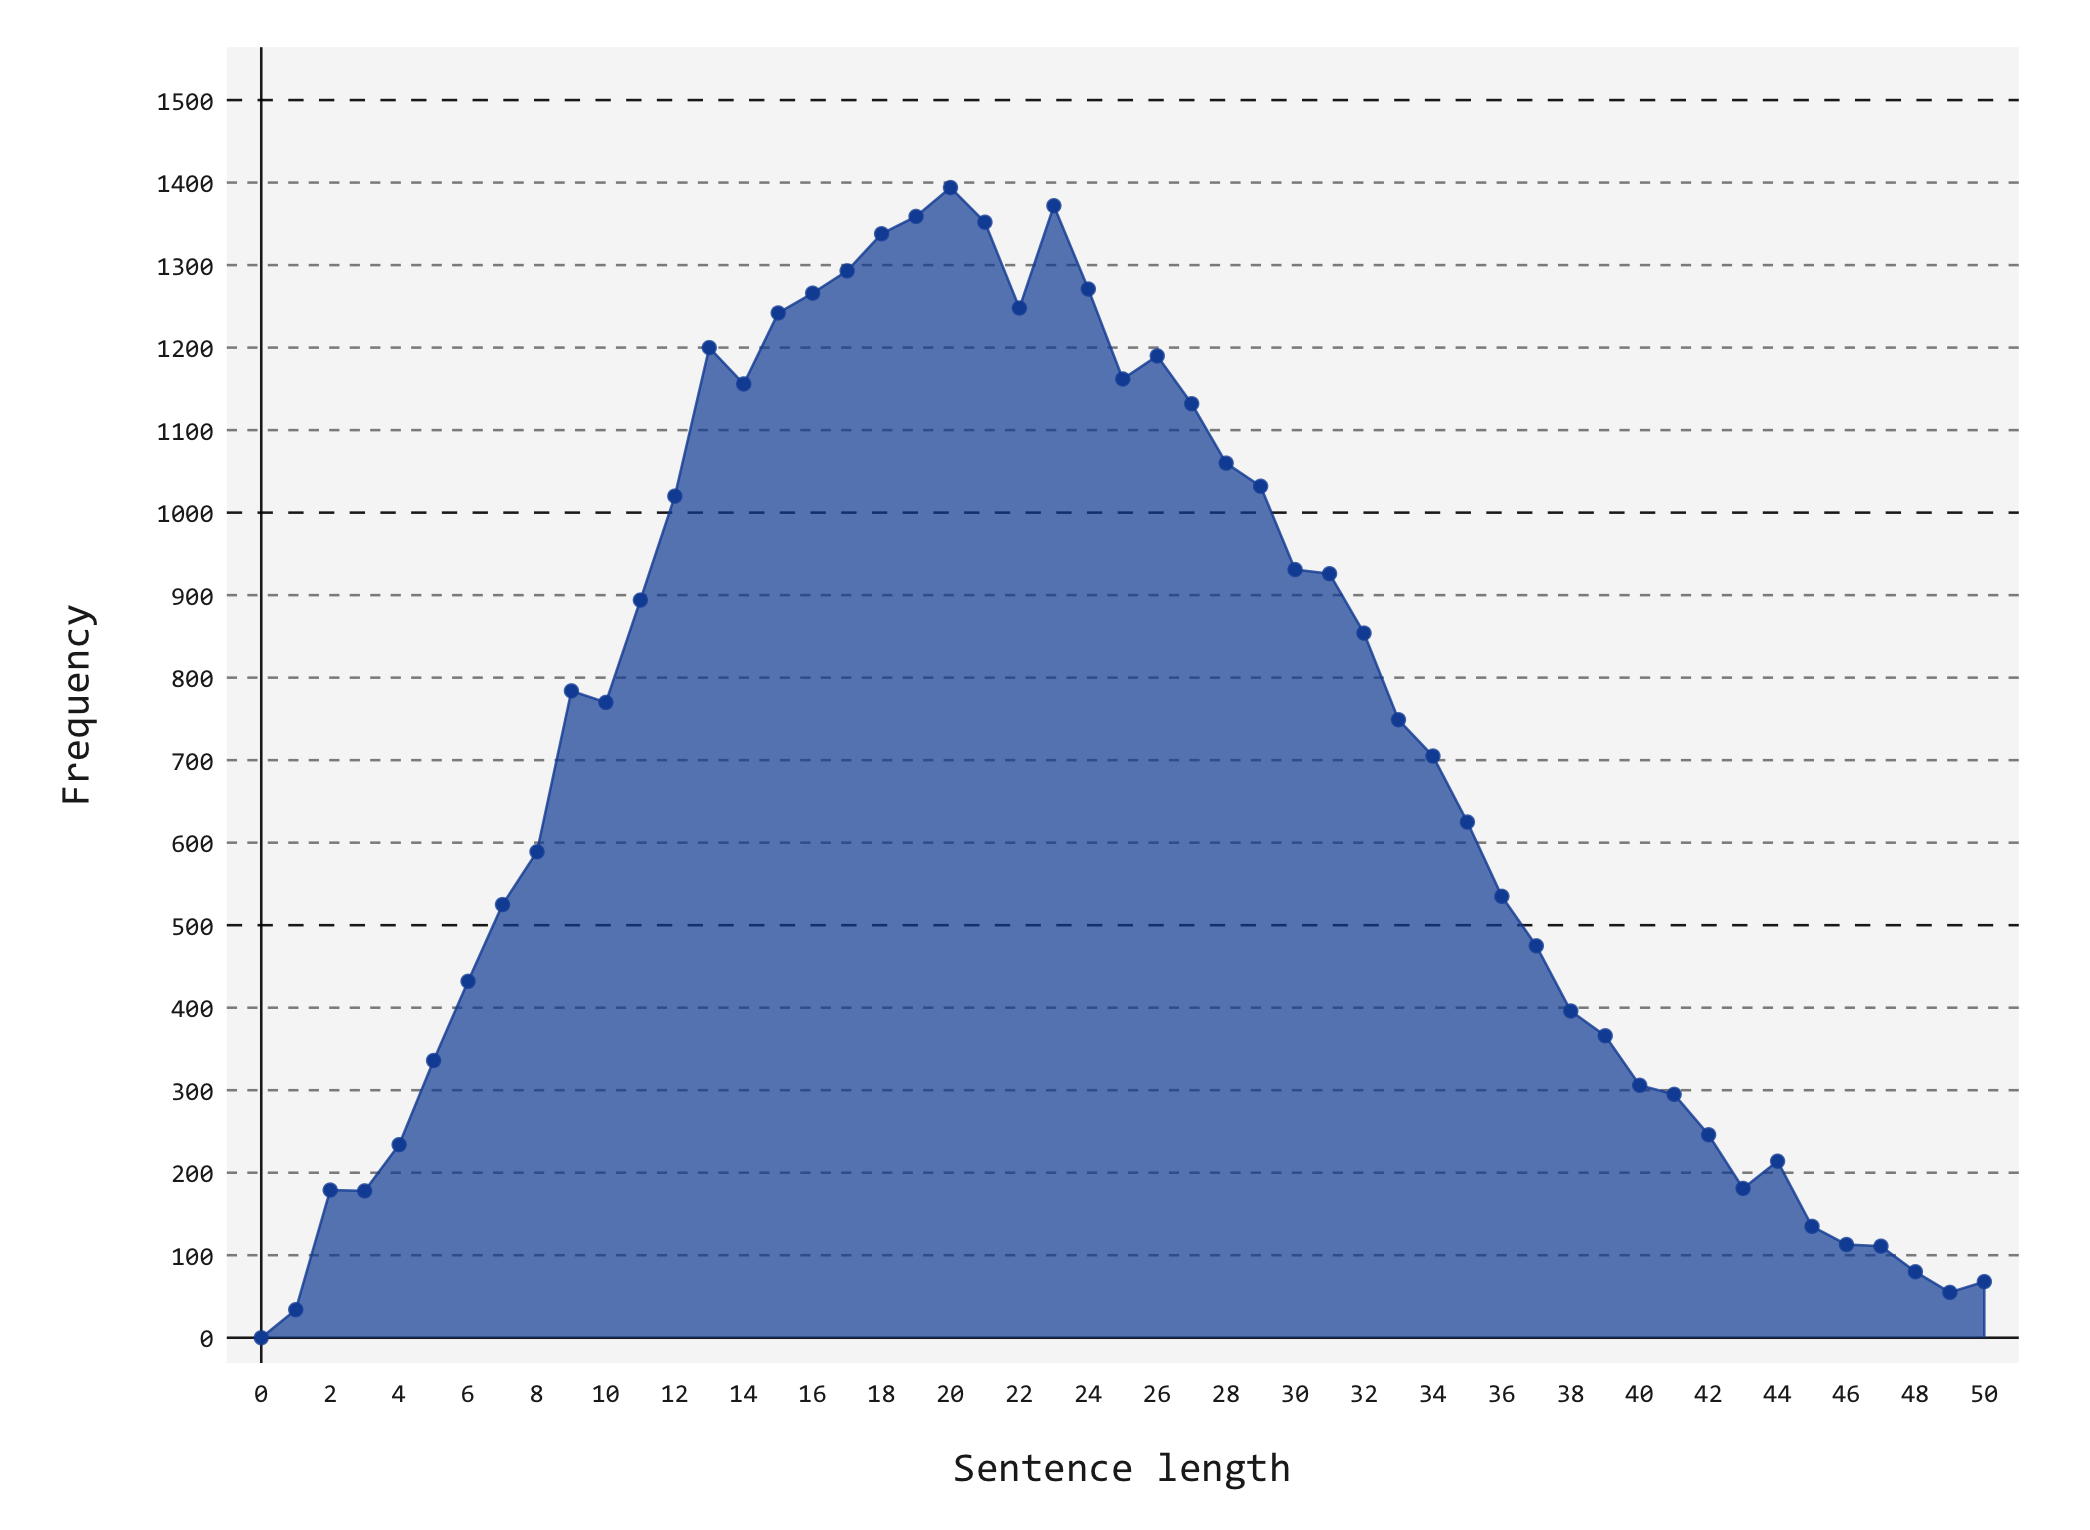
\includegraphics[width=\textwidth]{s_length_training}
    \end{minipage}\hfill
    \caption{Distribution of sentence lengths and their frequency in the training data.}
    \label{fig:sentence_length_1}
\end{figure}

\begin{figure}[h]
    \centering
    \begin{minipage}{0.8\textwidth}
        \centering
        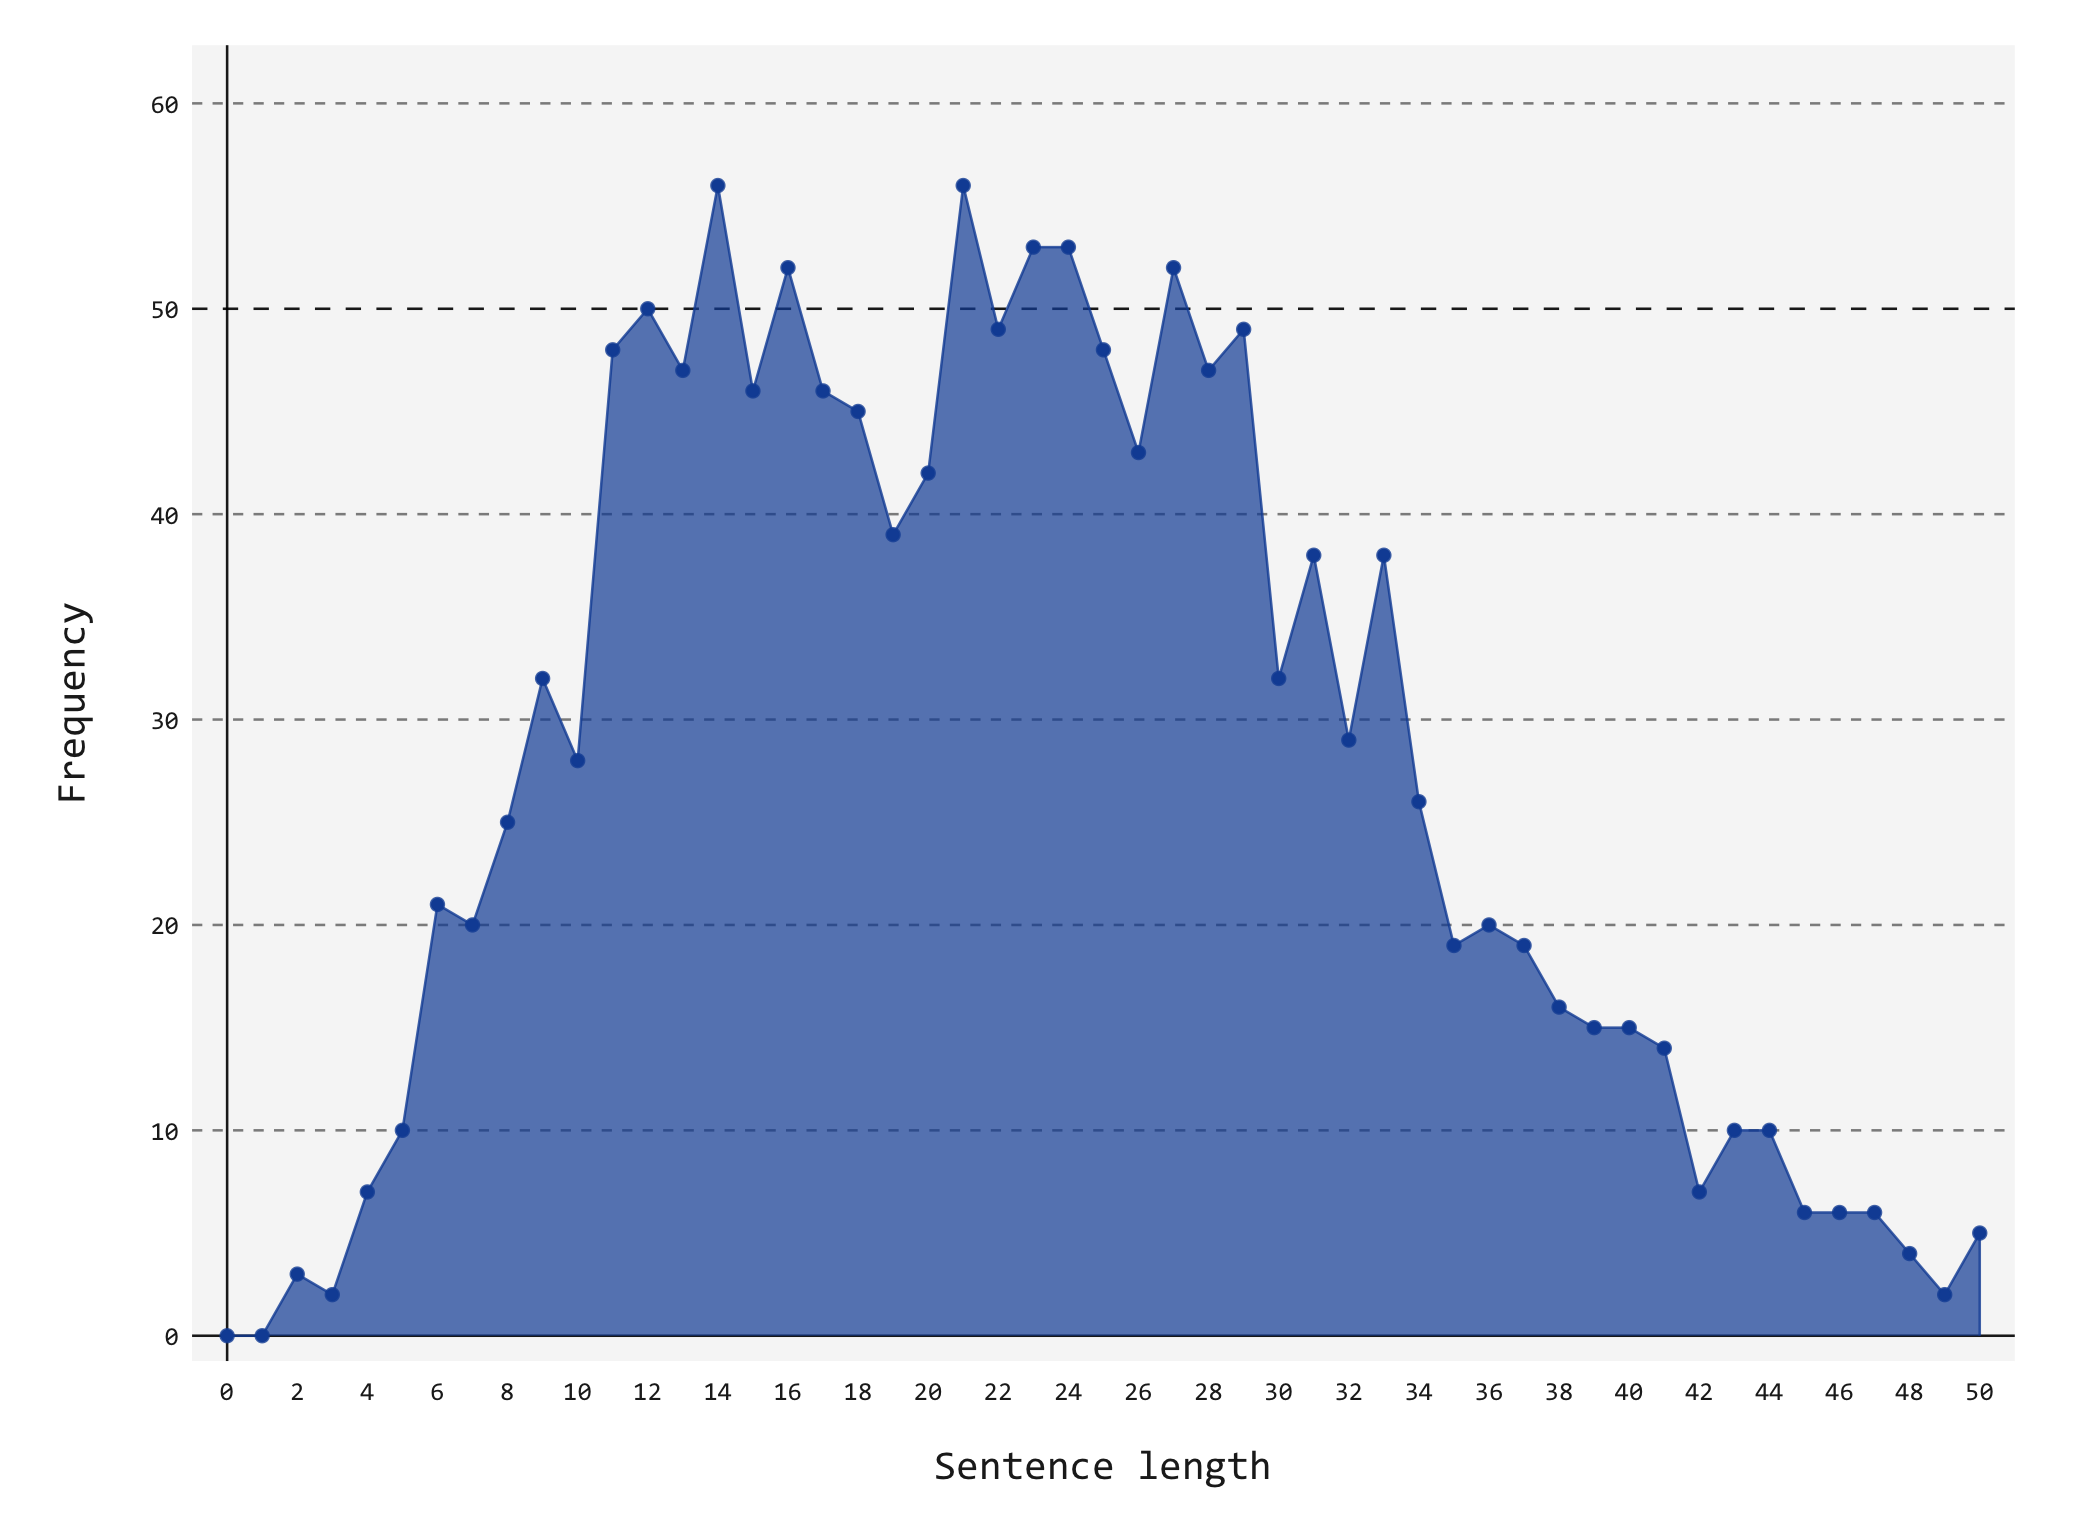
\includegraphics[width=\textwidth]{s_length_testing}
    \end{minipage}
    \caption{Distribution of sentence lengths and their frequency in the test data.}
    \label{fig:sentence_length_2}
\end{figure}

\begin{figure}[h]
    \centering
    \begin{minipage}{0.8\textwidth}
        \centering
        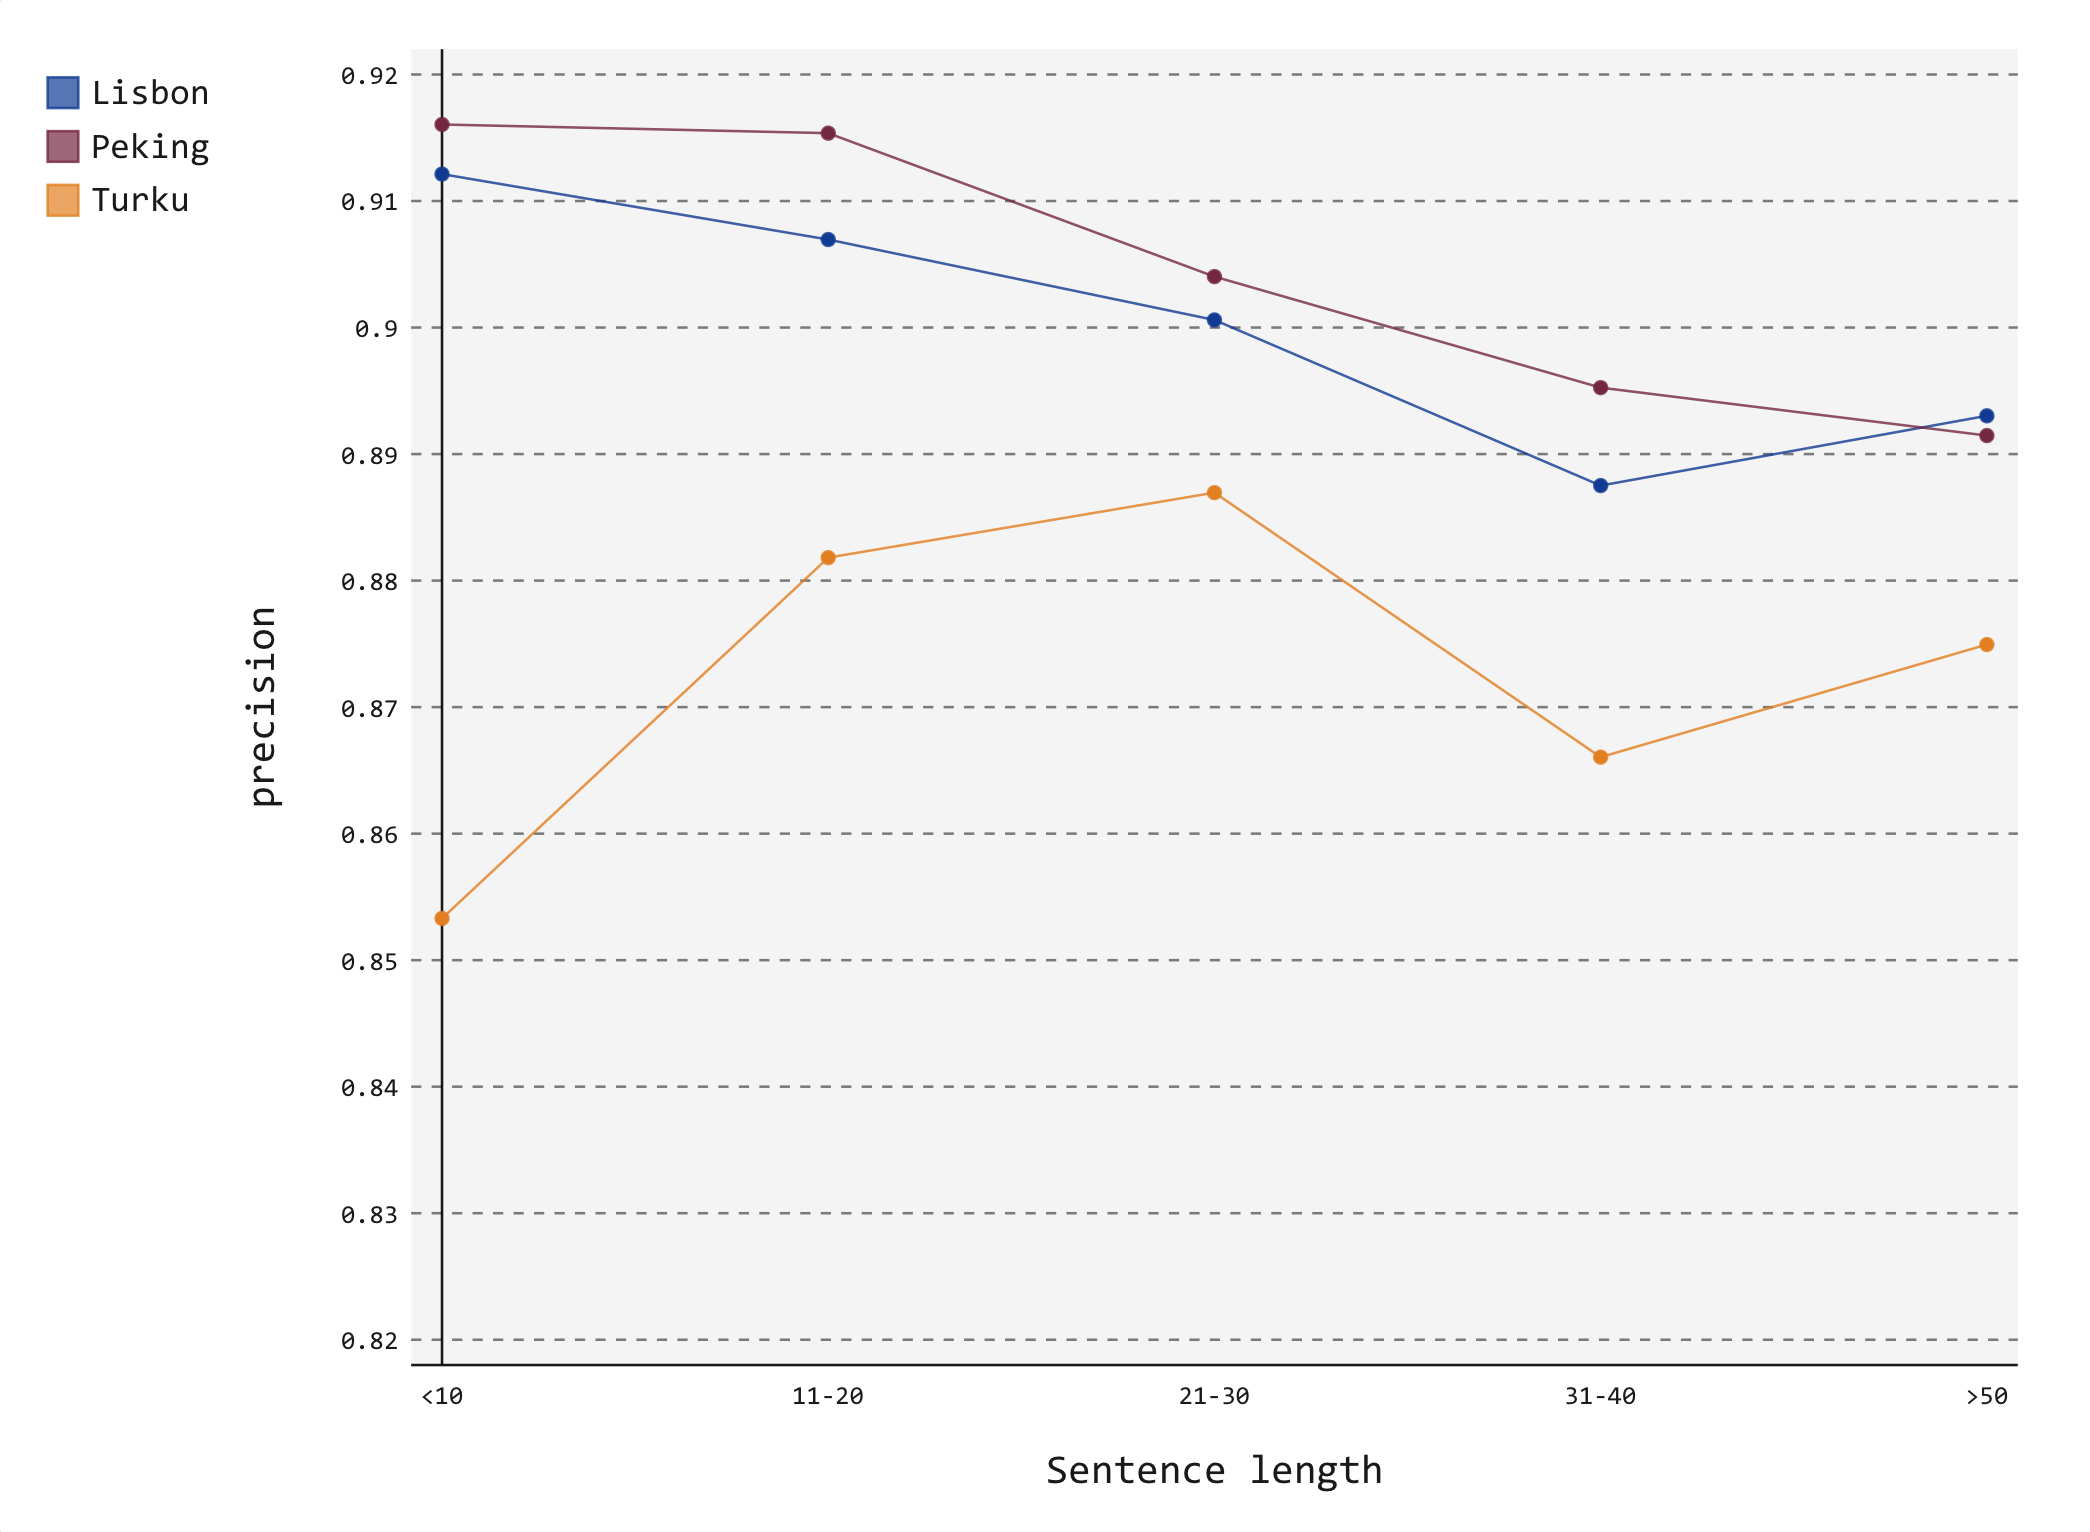
\includegraphics[width=\textwidth]{sentence_length_precision_DM}
    \end{minipage}
    \caption{Accuracy relative to sentence length in bins of size 10. Precision for the DM target representation.}
    \label{fig:s_length_DM}
\end{figure}

\begin{figure}[h]
    \centering
    \begin{minipage}{0.8\textwidth}
        \centering
        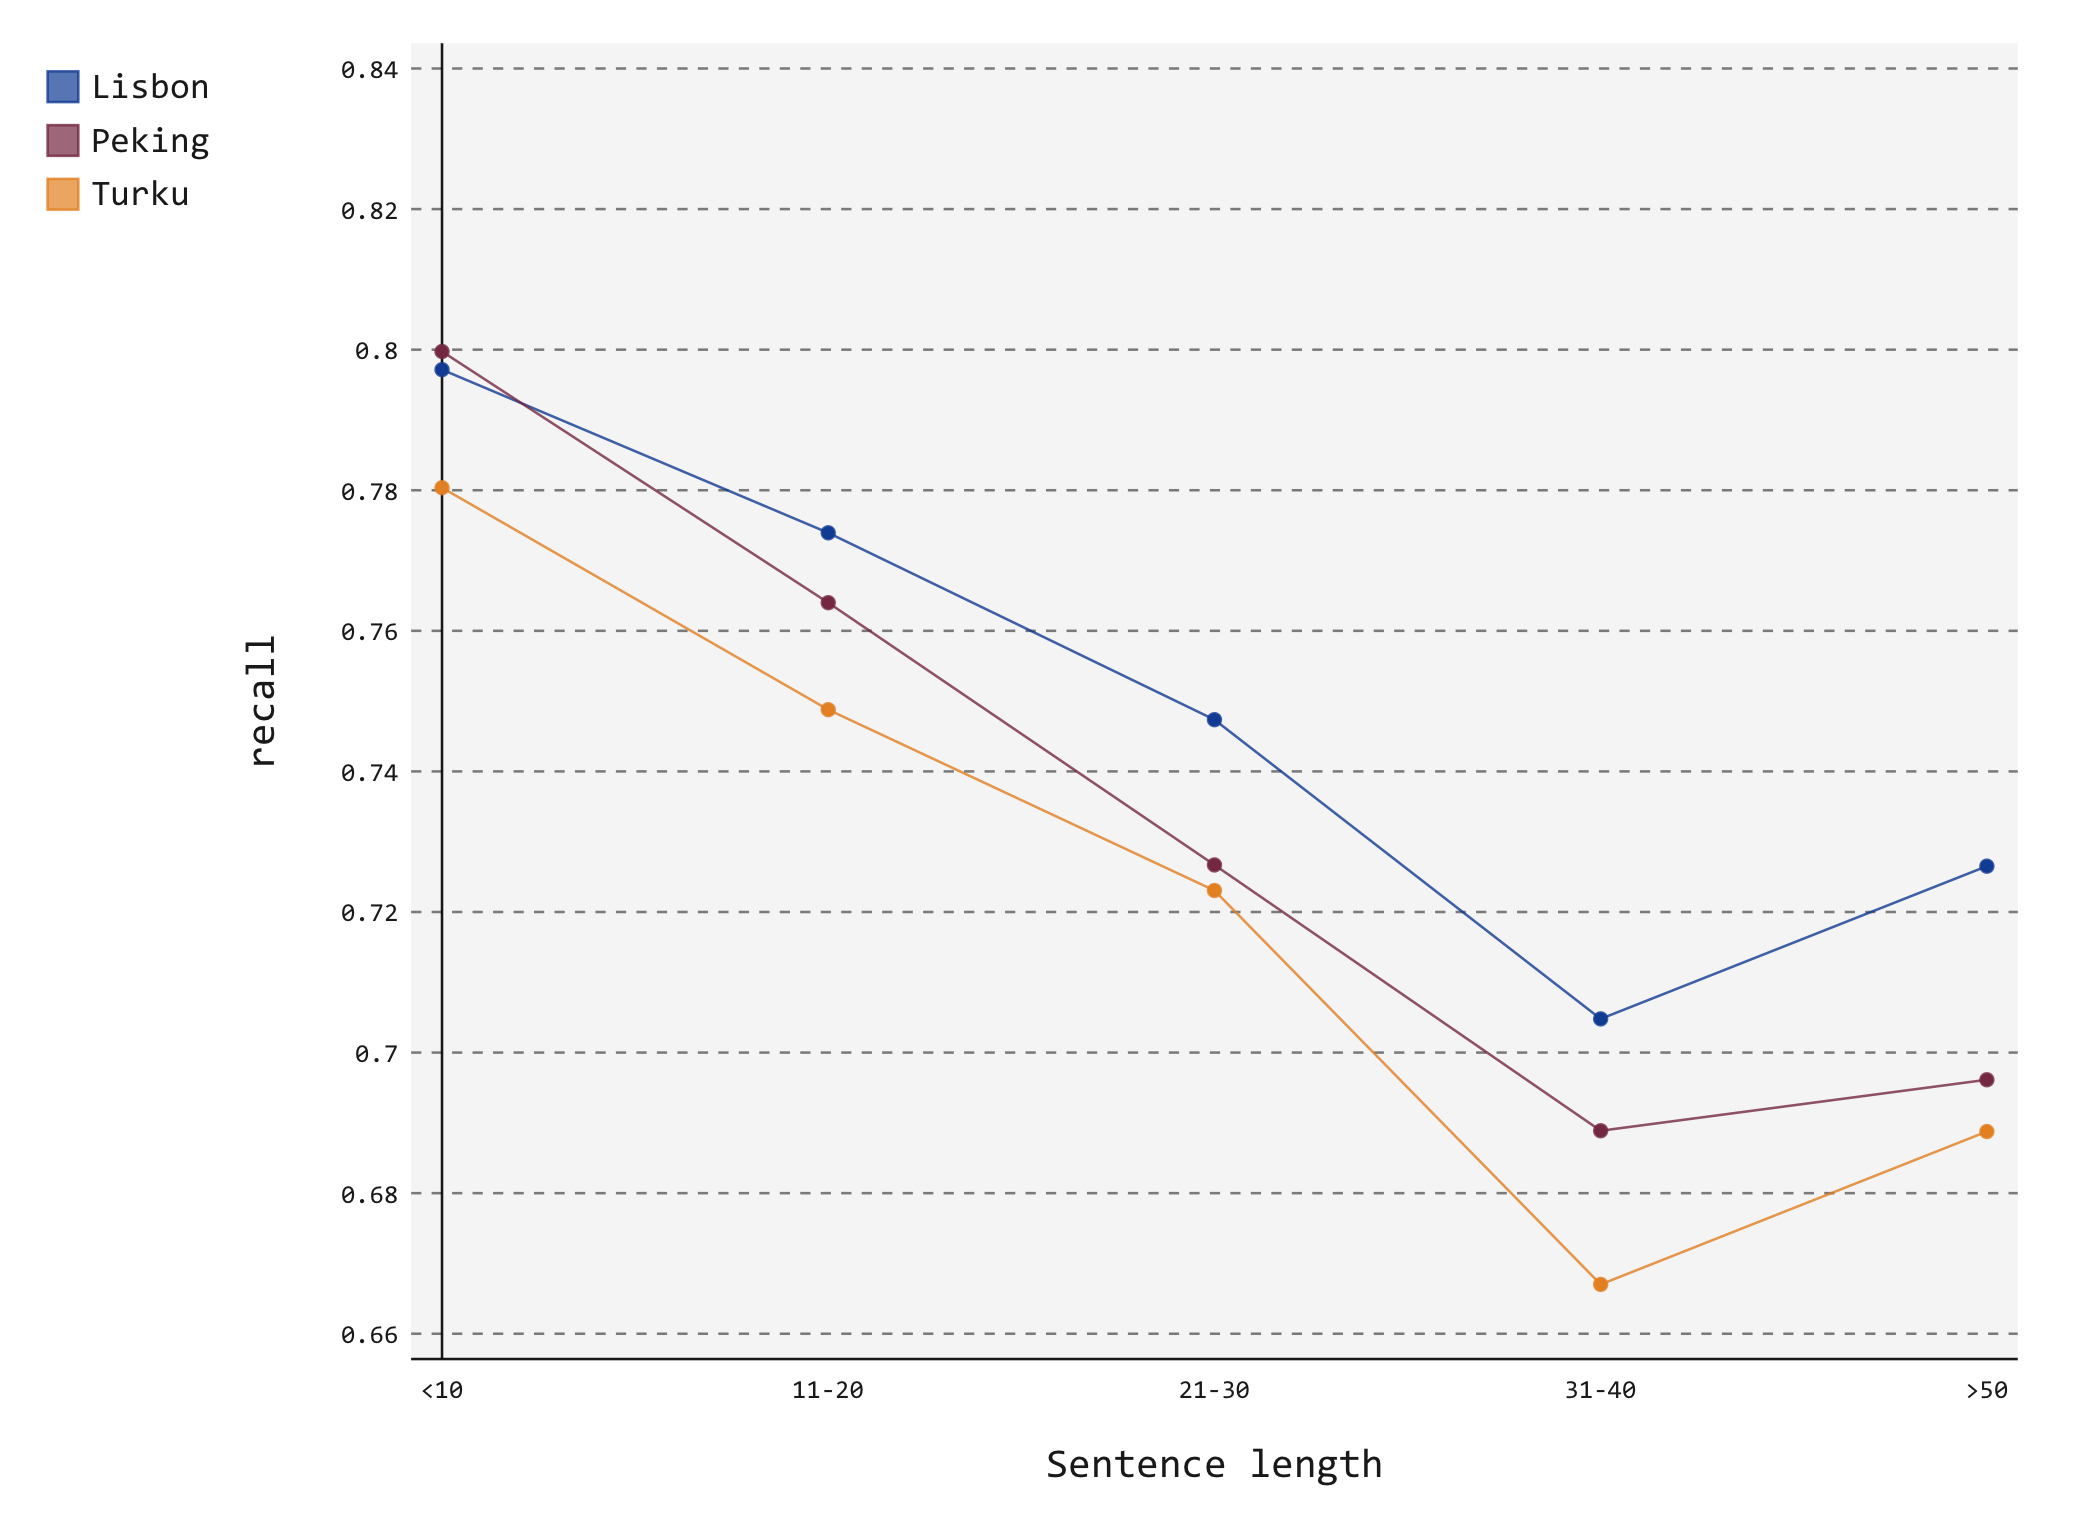
\includegraphics[width=\textwidth]{sentence_length_recall_PSD}
    \end{minipage}\hfill
    \caption{Accuracy relative to sentence length in bins of size 10. Recall for the PSD target representation.}
    \label{fig:s_length_PSD}
\end{figure}

In this section we will examine sentence length as a factor of parsing. First we point out the distribution of sentence lengths in the training and test data in Figure \ref{fig:sentence_length_1}, and \ref{fig:sentence_length_2} respectively. The distribution approximates the \textit{Bell curve}, and the average sentence length is 22.51 lexical units for the training, and 22.66 for the test data. However, the test data has a distribution where the approximation towards the Bell curve is more crude due to its relatively smaller size.

In Figures \ref{fig:s_length_DM} and \ref{fig:s_length_PSD} we see the precision and recall for the three parsing systems for sentence length. The graphs in these Figures show precision and recall for sentences in bins of 10. If we look at the DM target representation, we see that the results of Lisbon and Peking are quite similar, where there is a correlation of precision and recall in relation to sentence length. The overall trend is that for longer sentences, the precision and recall of the parsing decreases. This overall trend was also observed by \citeA{McD:Niv:07}, \citeA{McD:Niv:11}, and \citeA{Choi:Tetreaul:Stent:15} when examining syntactic parsers.

In comparison to the results from the syntactic dependency parsers examined in the studies of \citeA{McD:Niv:07}, \citeA{McD:Niv:11}, and \citeA{Choi:Tetreaul:Stent:15}, in our analysis we see a slight upwards bump in precision and recall for the last bin that includes sentences that are longer than 50 lexical units. This can be explained by the fact that there are very few sentences with more than 50 lexical units in the testing data set, and that a slight bump might be attributed to the relatively smaller size of that bin. It is therefore worth noting that changing bin sizes would give us slightly different graphs, but that the overall trend would nonetheless be a slight decrease in accuracy as sentence lengths grow.

Another factor that can impact the bump in the last bin is that for semantic dependency graphs we might actually be dealing with two or more disjoint graphs. For sentences that have more than 50 lexical units, a sentence might produce a semantic dependency graph that would be similar to that of two sentences, and we thus would expect a higher accuracy on the combined accuracy. This would not be possible in syntactic dependency parsers, where we don't have the possibility of disjoint trees.

Studying the graphs in Figures \ref{fig:s_length_DM} and \ref{fig:s_length_PSD}, we observe that the Lisbon and Peking systems share quite a similar trajectory for both the DM and PSD target representations, with only subtle differences. The Peking parsing system performs better on the DM target representation, while the Lisbon parsing system performs better on the PSD target representation. However, for sentences smaller than 10 lexical units, the Peking parsing system has a higher precision and recall than Lisbon on the PSD target representation. On the DM target representation the trend is opposite; the Lisbon parsing system outperforms Peking on sentences that are longer than 50 lexical units. These difference might be attributed to the differences in the technical aspects of these parsing systems.

The Lisbon parsing systems use a technique where several graphs are created, and then an approximation is used to select the highest scoring graph. For longer sentences this technique may result in higher accuracy as may be more capable of producing the disjoint graphs that are possible for longer sentences. See \citeA{Mar:Al:Lisbon:14} for a detailed description. The Peking system, on the other hand, use a transition based model, and as such longer sentences can be more challenging. 

Turku on the other hand has an overall different trajectory in comparison to the other two parsing systems on the DM target representation. The largest deviation from the overall trend is that the Turku system, when parsing on the DM target representation, show a particularly low precision and recall on sentences that have lower than 10 lexical units. This is not present when parsing on the PSD target representation, and should be considered an anomaly that might be attributed to some technical detail of the Turku parsing system. Since the Turku parsing system uses a Support Vector Machine for its parsing, shorter sentences might pose an issue if the features use depend on more information than what is present for shorter sentences. More analysis is needed in order to clarify the reasoning behind this anomaly in the Turku parsing system.


% In Figures \ref{fig:dm_s_length} and \ref{fig:psd_s_length}, we have graphs for the precision and recall of the three parsing systems for both the DM and SDP target representations. As \citeA{McD:Niv:07}, \citeA{McD:Niv:11}, and \citeA{Choi:Tetreaul:Stent:15} found when examining various syntactic parsers, there is also a correlation between sentence length and the accuracy of semantic dependency parsing systems. The longer the sentence, the lower the precision and recall of the results.

% If we look at Figure \ref{fig:dm_s_length}, we see a sharp increase from sentences consisting of more than 3 to 5 lexical units, and then an overall slight reduction of precision and recall as we get longer sentences. We can also observe that the recall is affected to a higher degree than precision, indicating that at parsing, the produced graphs have more dependencies than the gold standard. 

% The correlation between sentence length and precision/recal is more prevalent for the PSD target representation. If we go back to Figure \label{fig:data} from Chapter \ref{chap:semantic}, we see that the PSD target representation has 91 labels, whereas DM has 59. This accounts for some of the reduction in precision and recall that we observe in the results on these two target representations. Examining Figure \ref{fig:psd_s_length}, we see that there is a steeper reduction in both precision and recall for PSD in comparison to DM. We can possibly conclude that the number of dependency types, i.e. the coarseness vs fineness of the dependencies, has a marked impact on the results of parsing systems. This is something that we return to below. 

% Sentence lengths

\subsection{Dependency length}

\begin{figure}[h]
    \centering
    \begin{minipage}{0.8\textwidth}
        \centering
        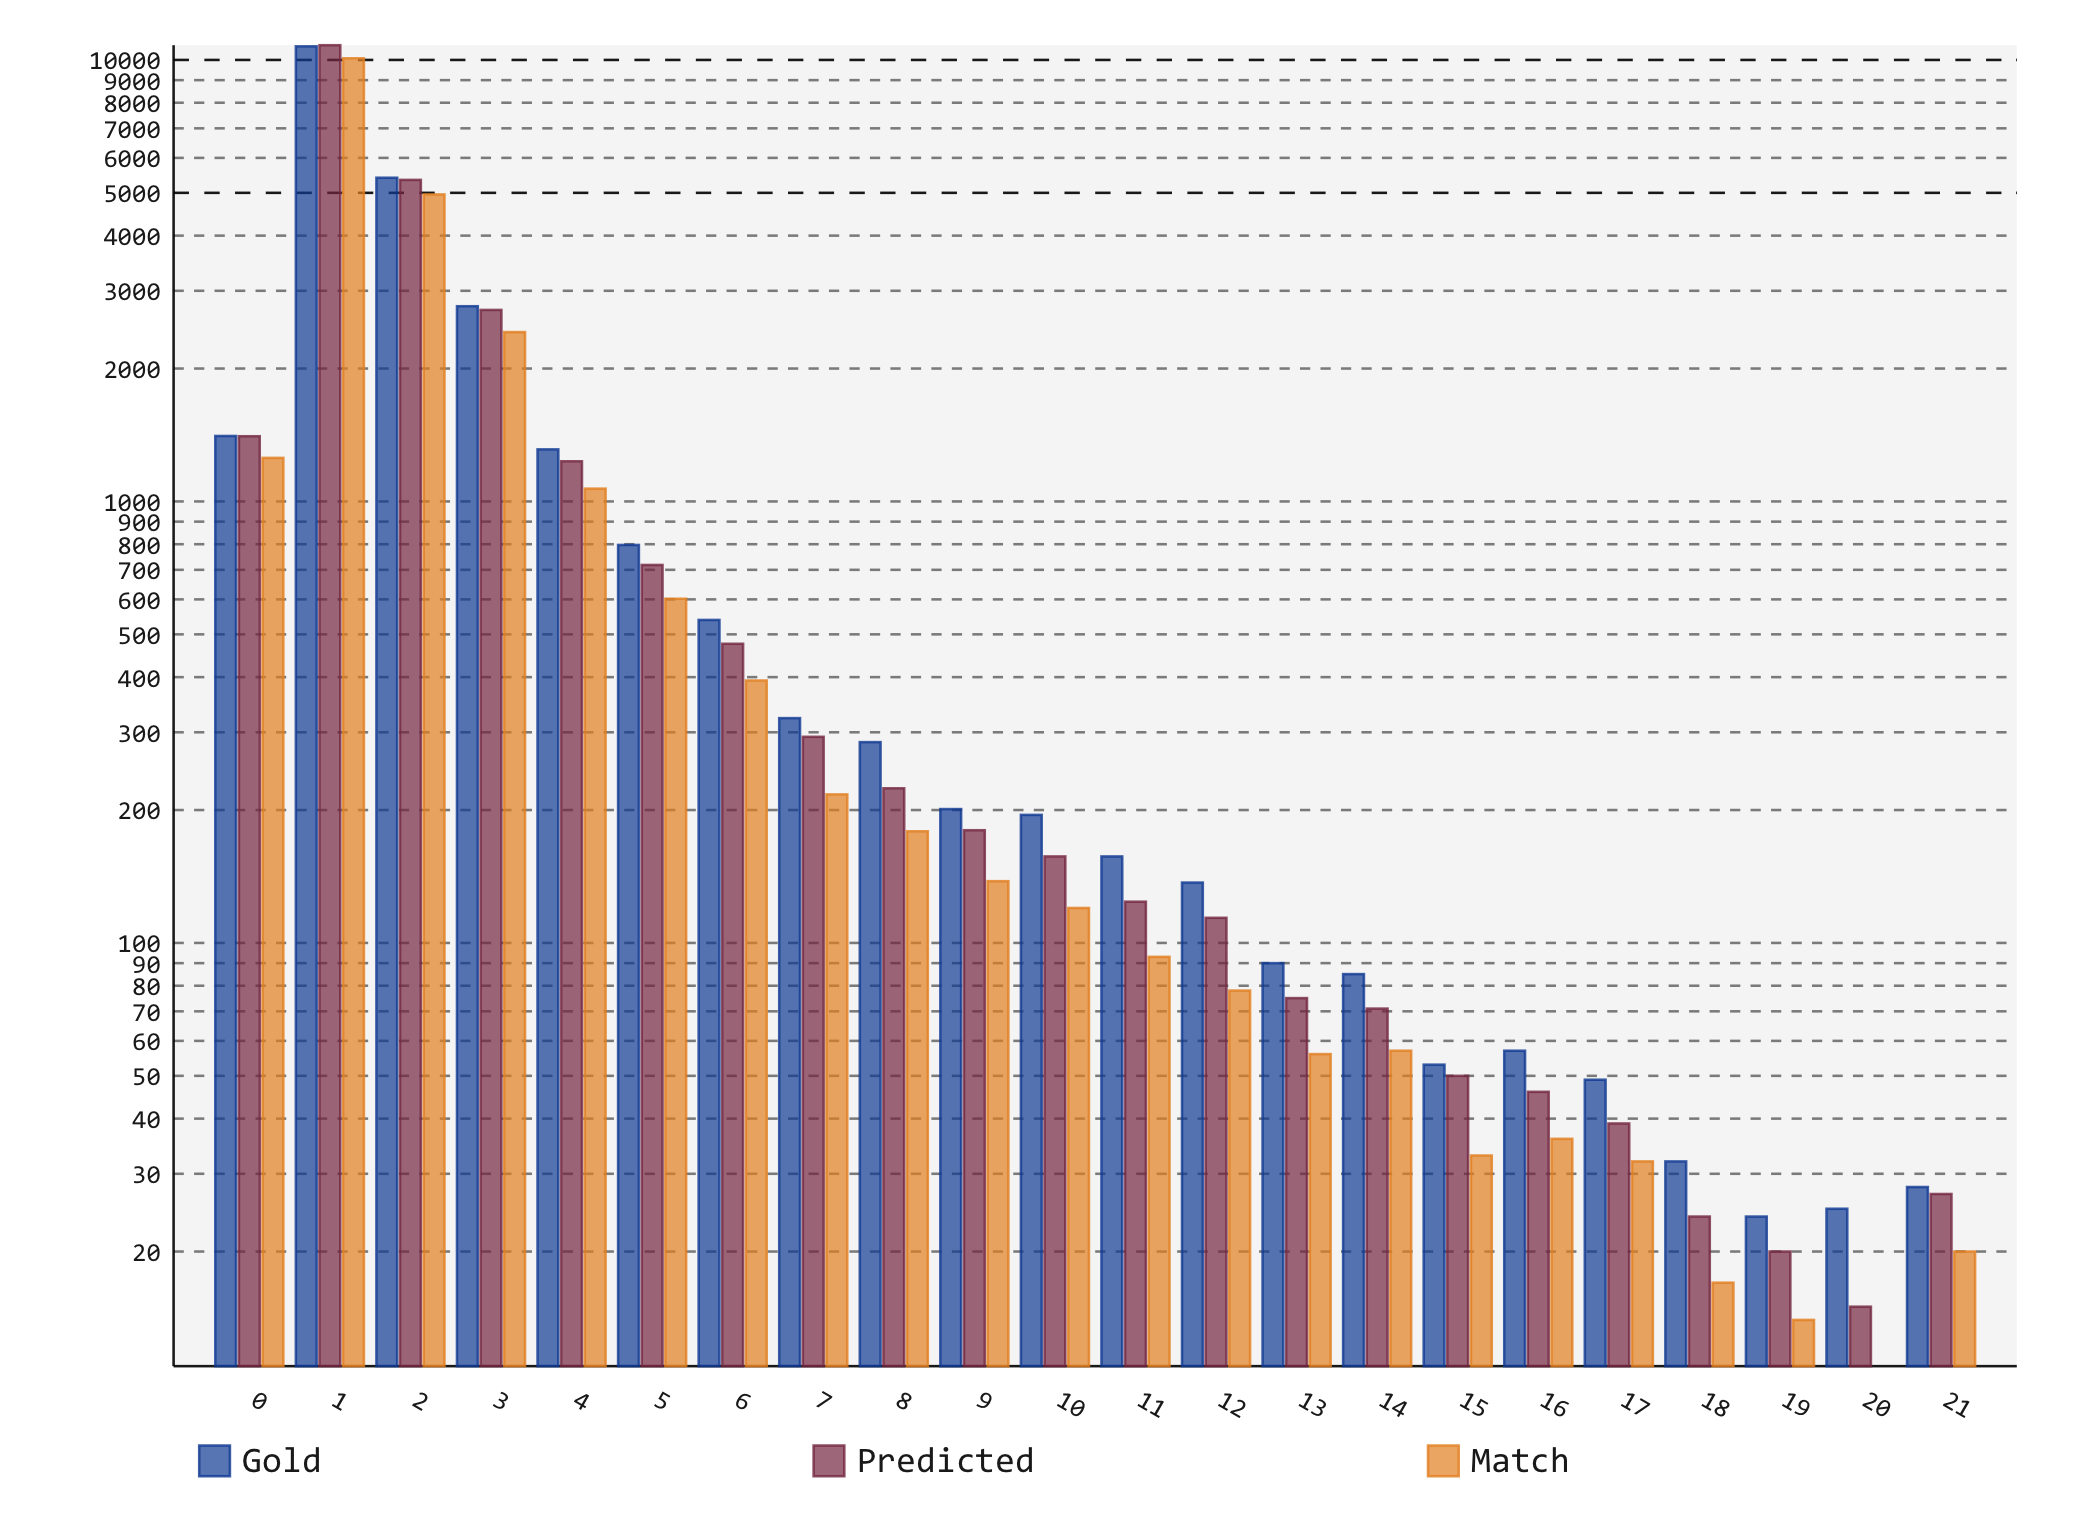
\includegraphics[width=\textwidth]{Lisbon_dep_len_DM}
    \end{minipage}\hfill
    \caption{The number of dependencies for the Lisbon parsing system according to their length (where 0 denotes top nodes) for the DM target representation. The graph shows the number of dependencies in the gold data set, the predicted dependencies, and the matches between predicted and gold.}
    \label{fig:Lisbon_dep_len_DM}
\end{figure}

\begin{figure}[h]
    \centering
    \begin{minipage}{0.8\textwidth}
        \centering
        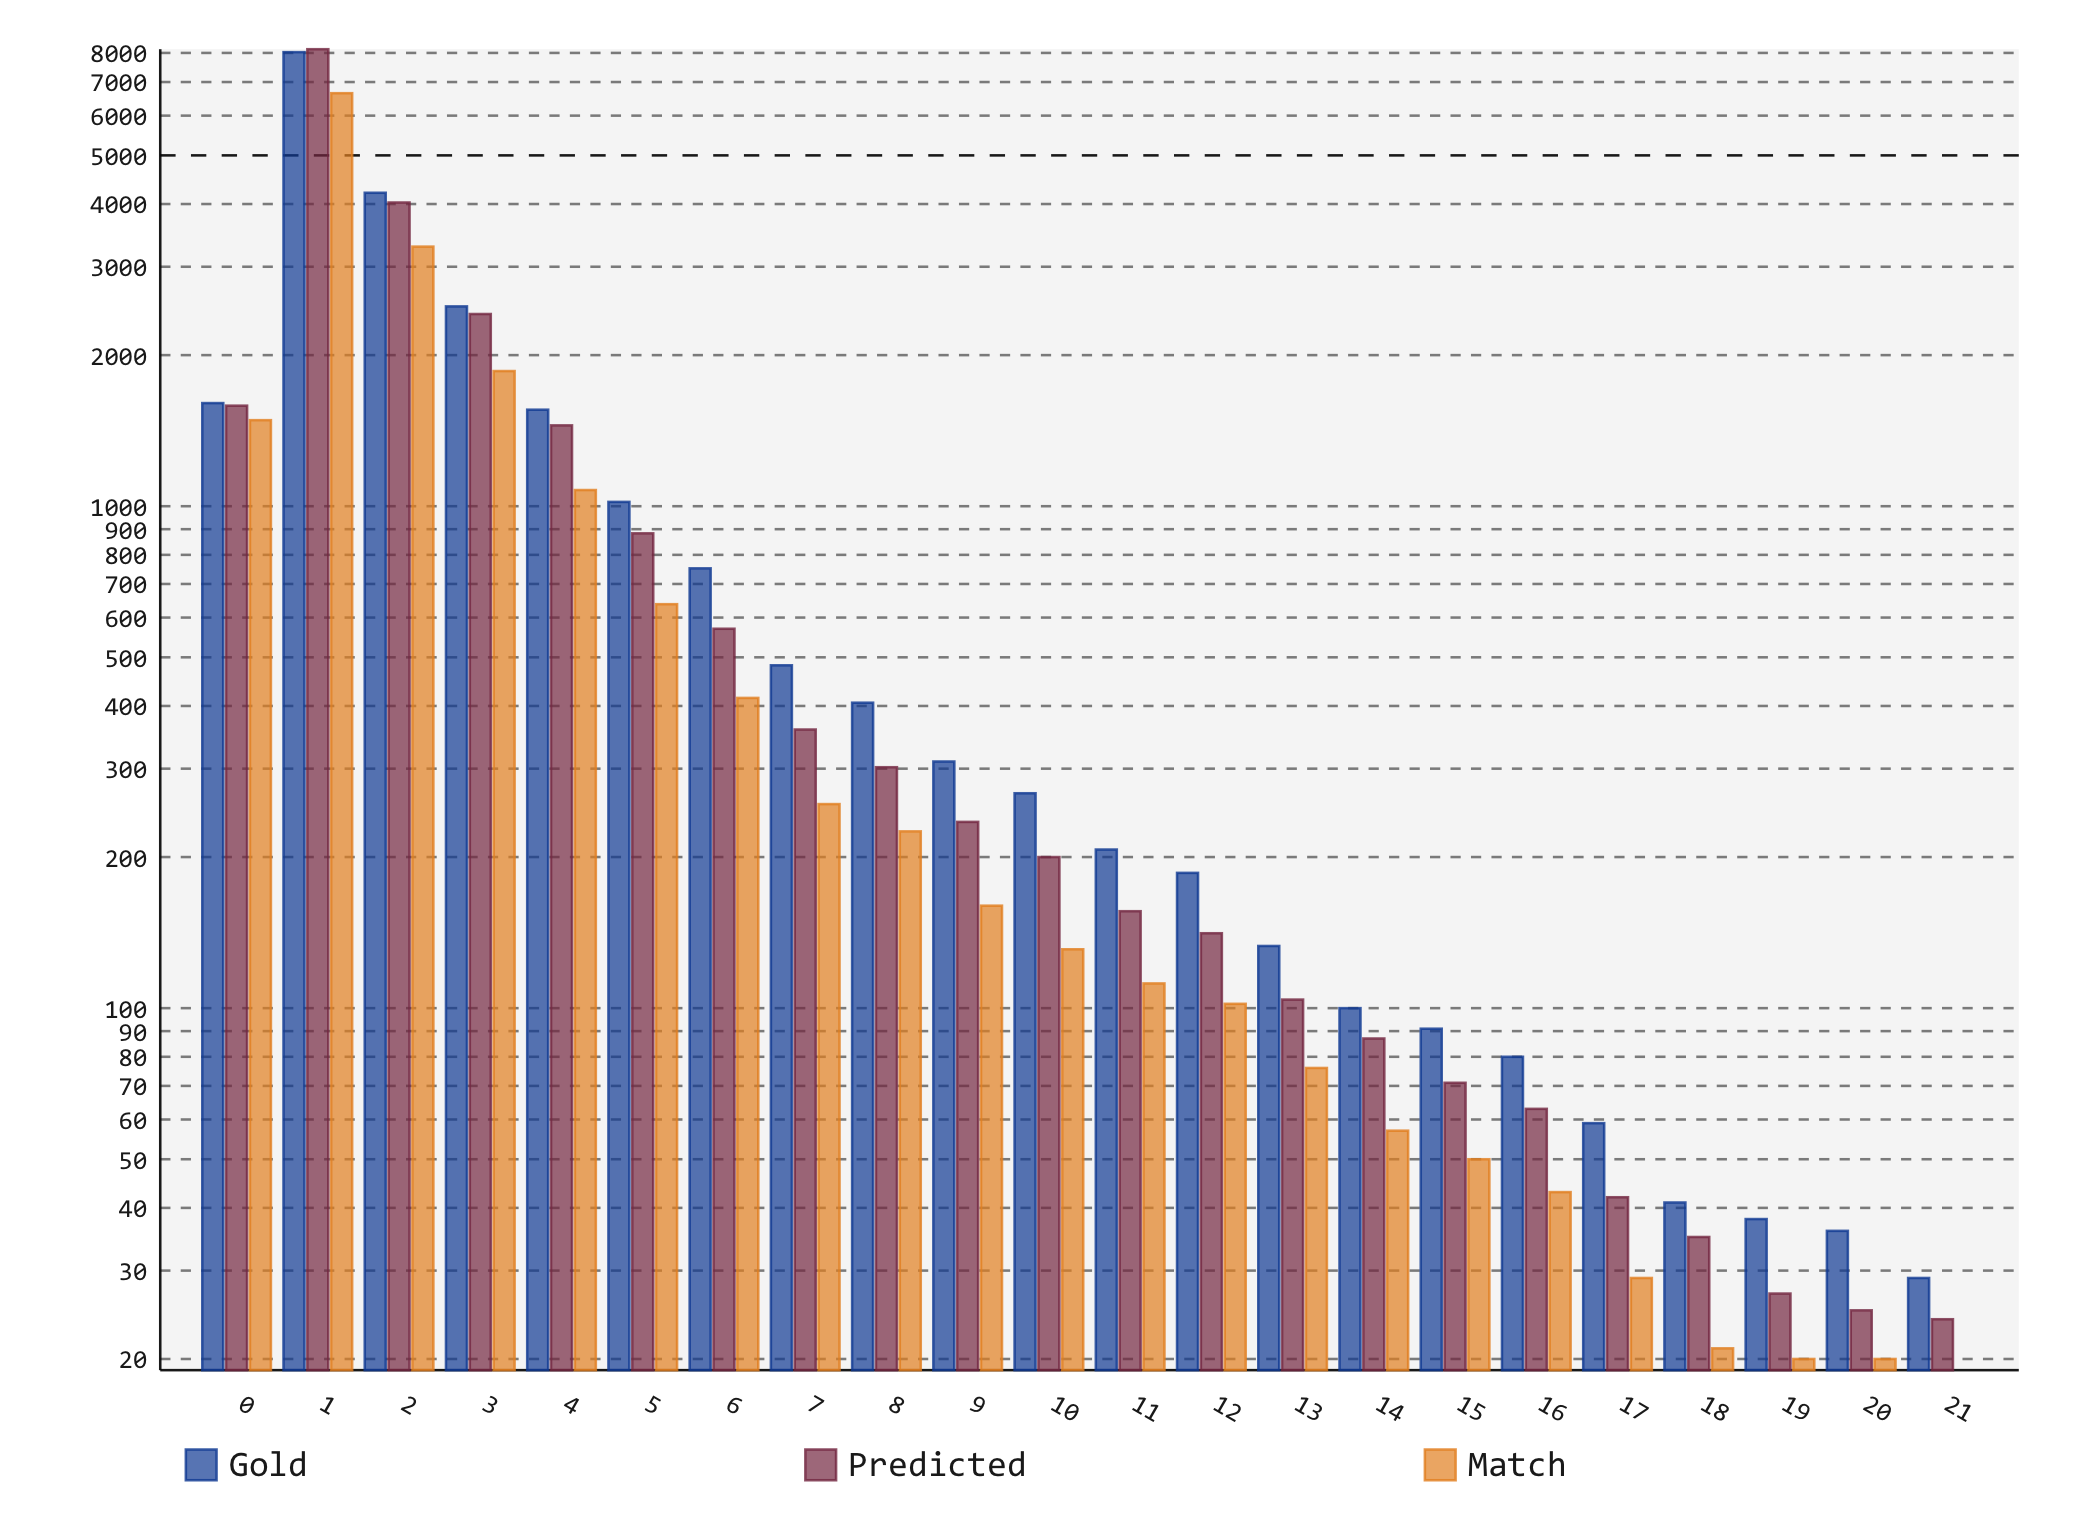
\includegraphics[width=\textwidth]{Lisbon_dep_len_PSD}
    \end{minipage}
    \caption{The number of dependencies for the Lisbon parsing system according to their length (where 0 denotes top nodes) for the PSD target representation. The graph shows the number of dependencies in the gold data set, the predicted dependencies, and the matches between predicted and gold.}
    \label{fig:Lisbon_dep_len_PSD}
\end{figure}

\begin{figure}[h]
    \centering
    \begin{minipage}{0.8\textwidth}
        \centering
        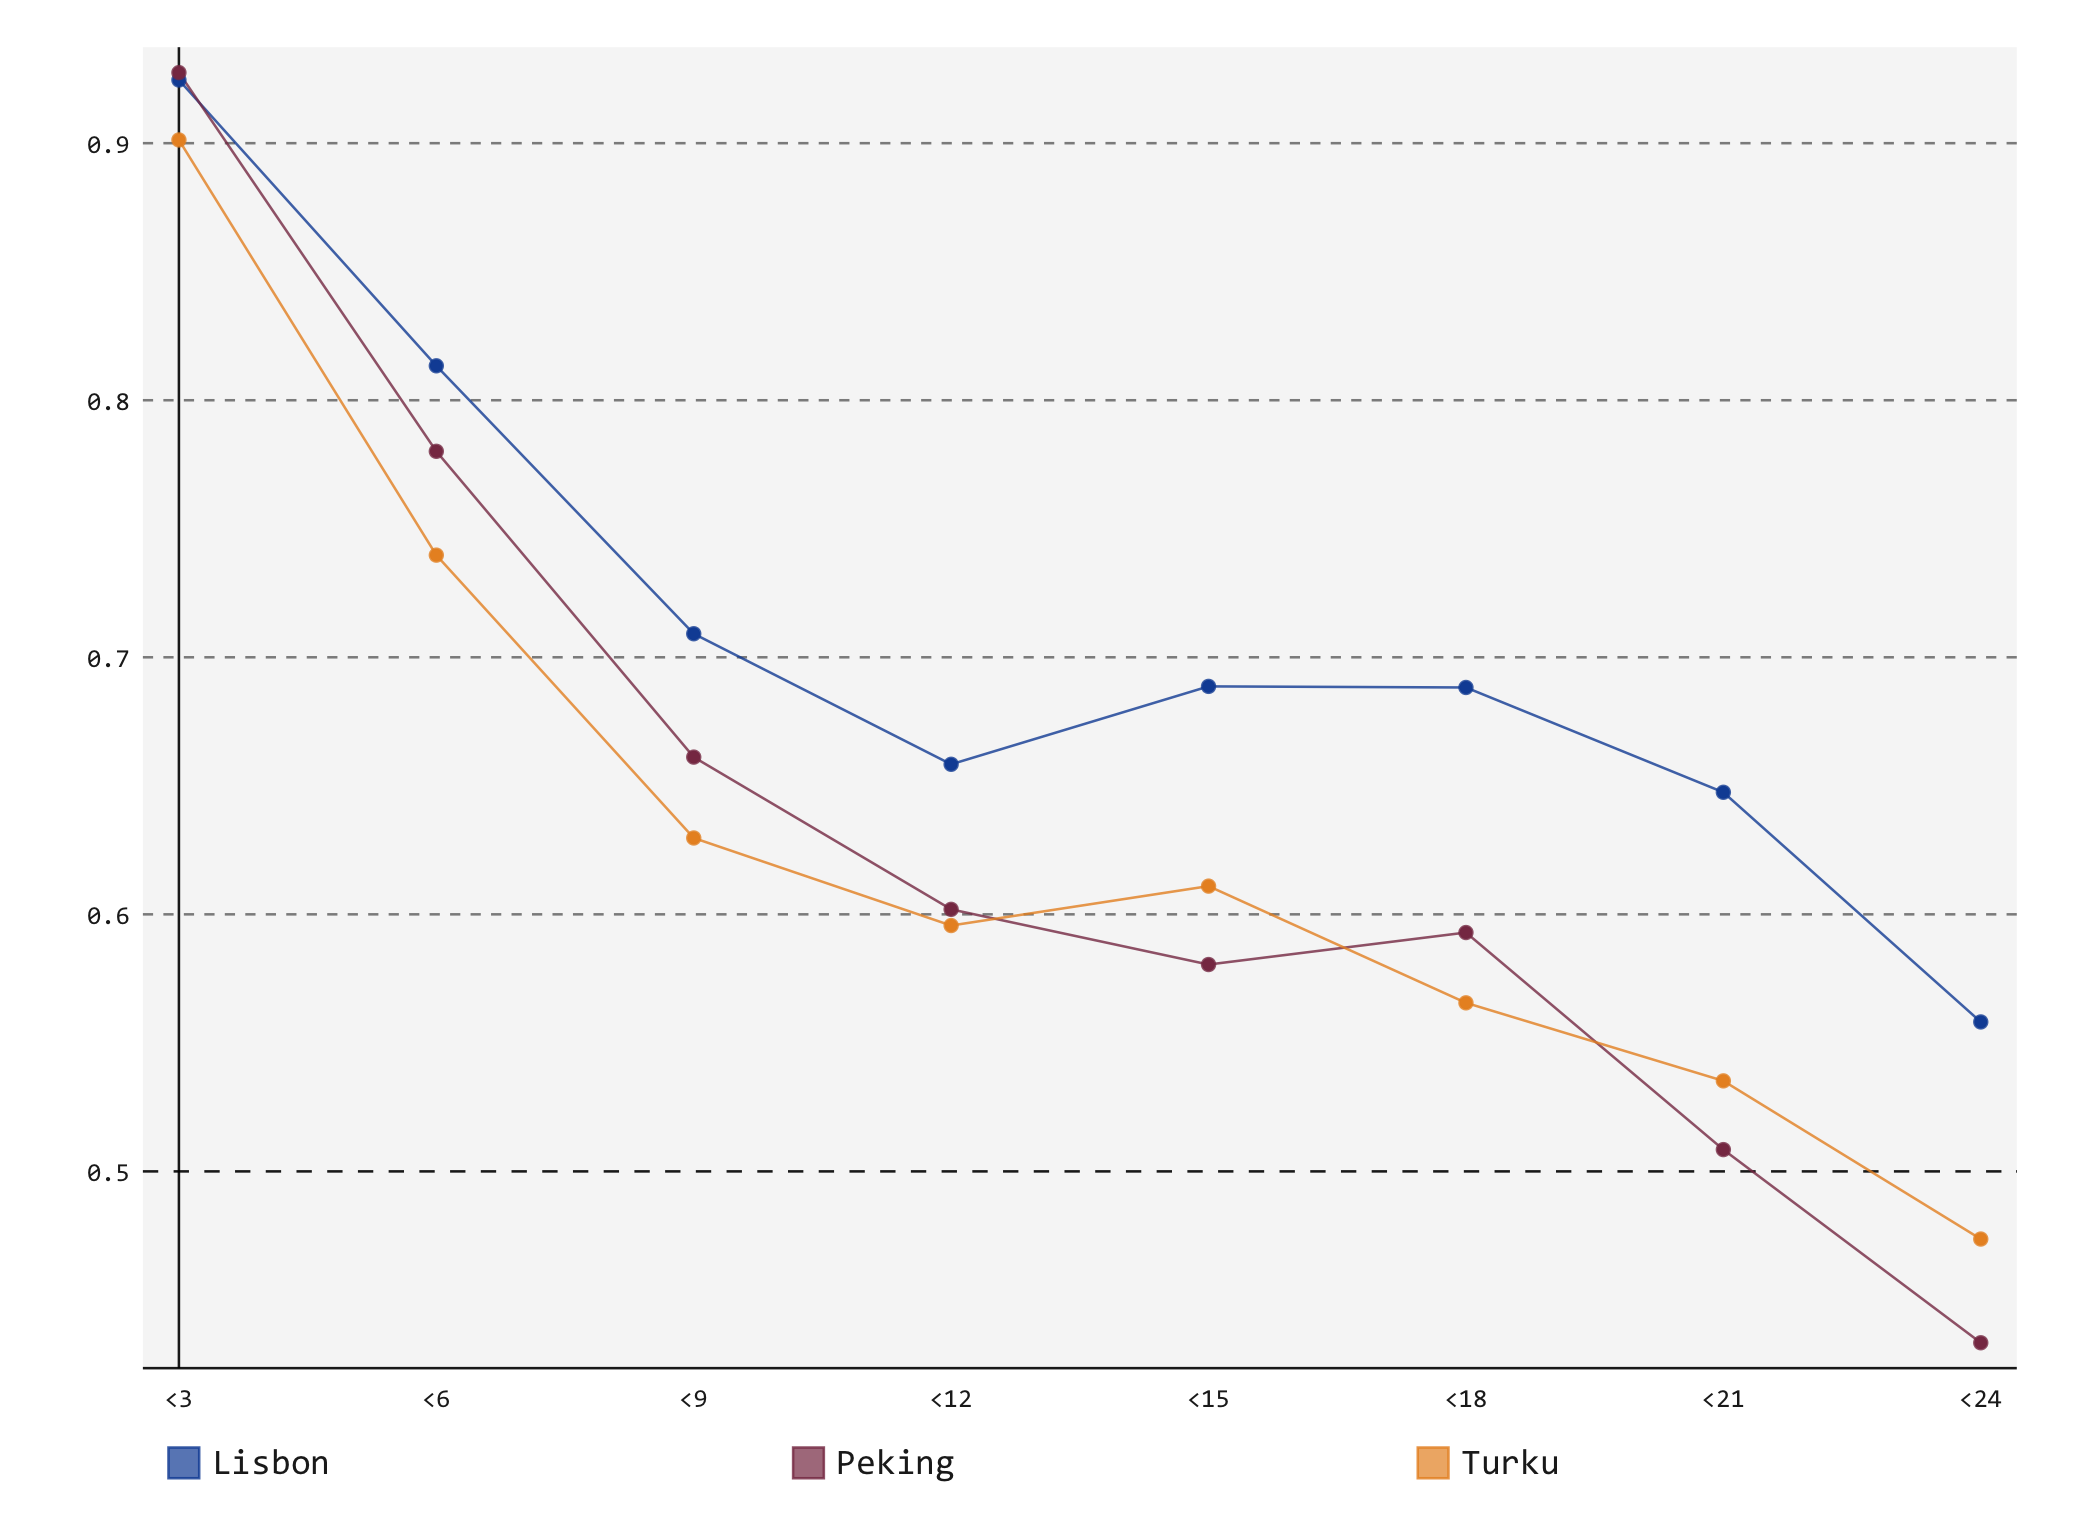
\includegraphics[width=\textwidth]{dep_len_fscore_DM}
    \end{minipage}\hfill
    \caption{F-score for the three parsing systems on the DM target representations for dependency length in bins of 3.}
    \label{fig:dep_len_fscore_DM}
\end{figure}

\begin{figure}[h]
    \centering
    \begin{minipage}{0.8\textwidth}
        \centering
        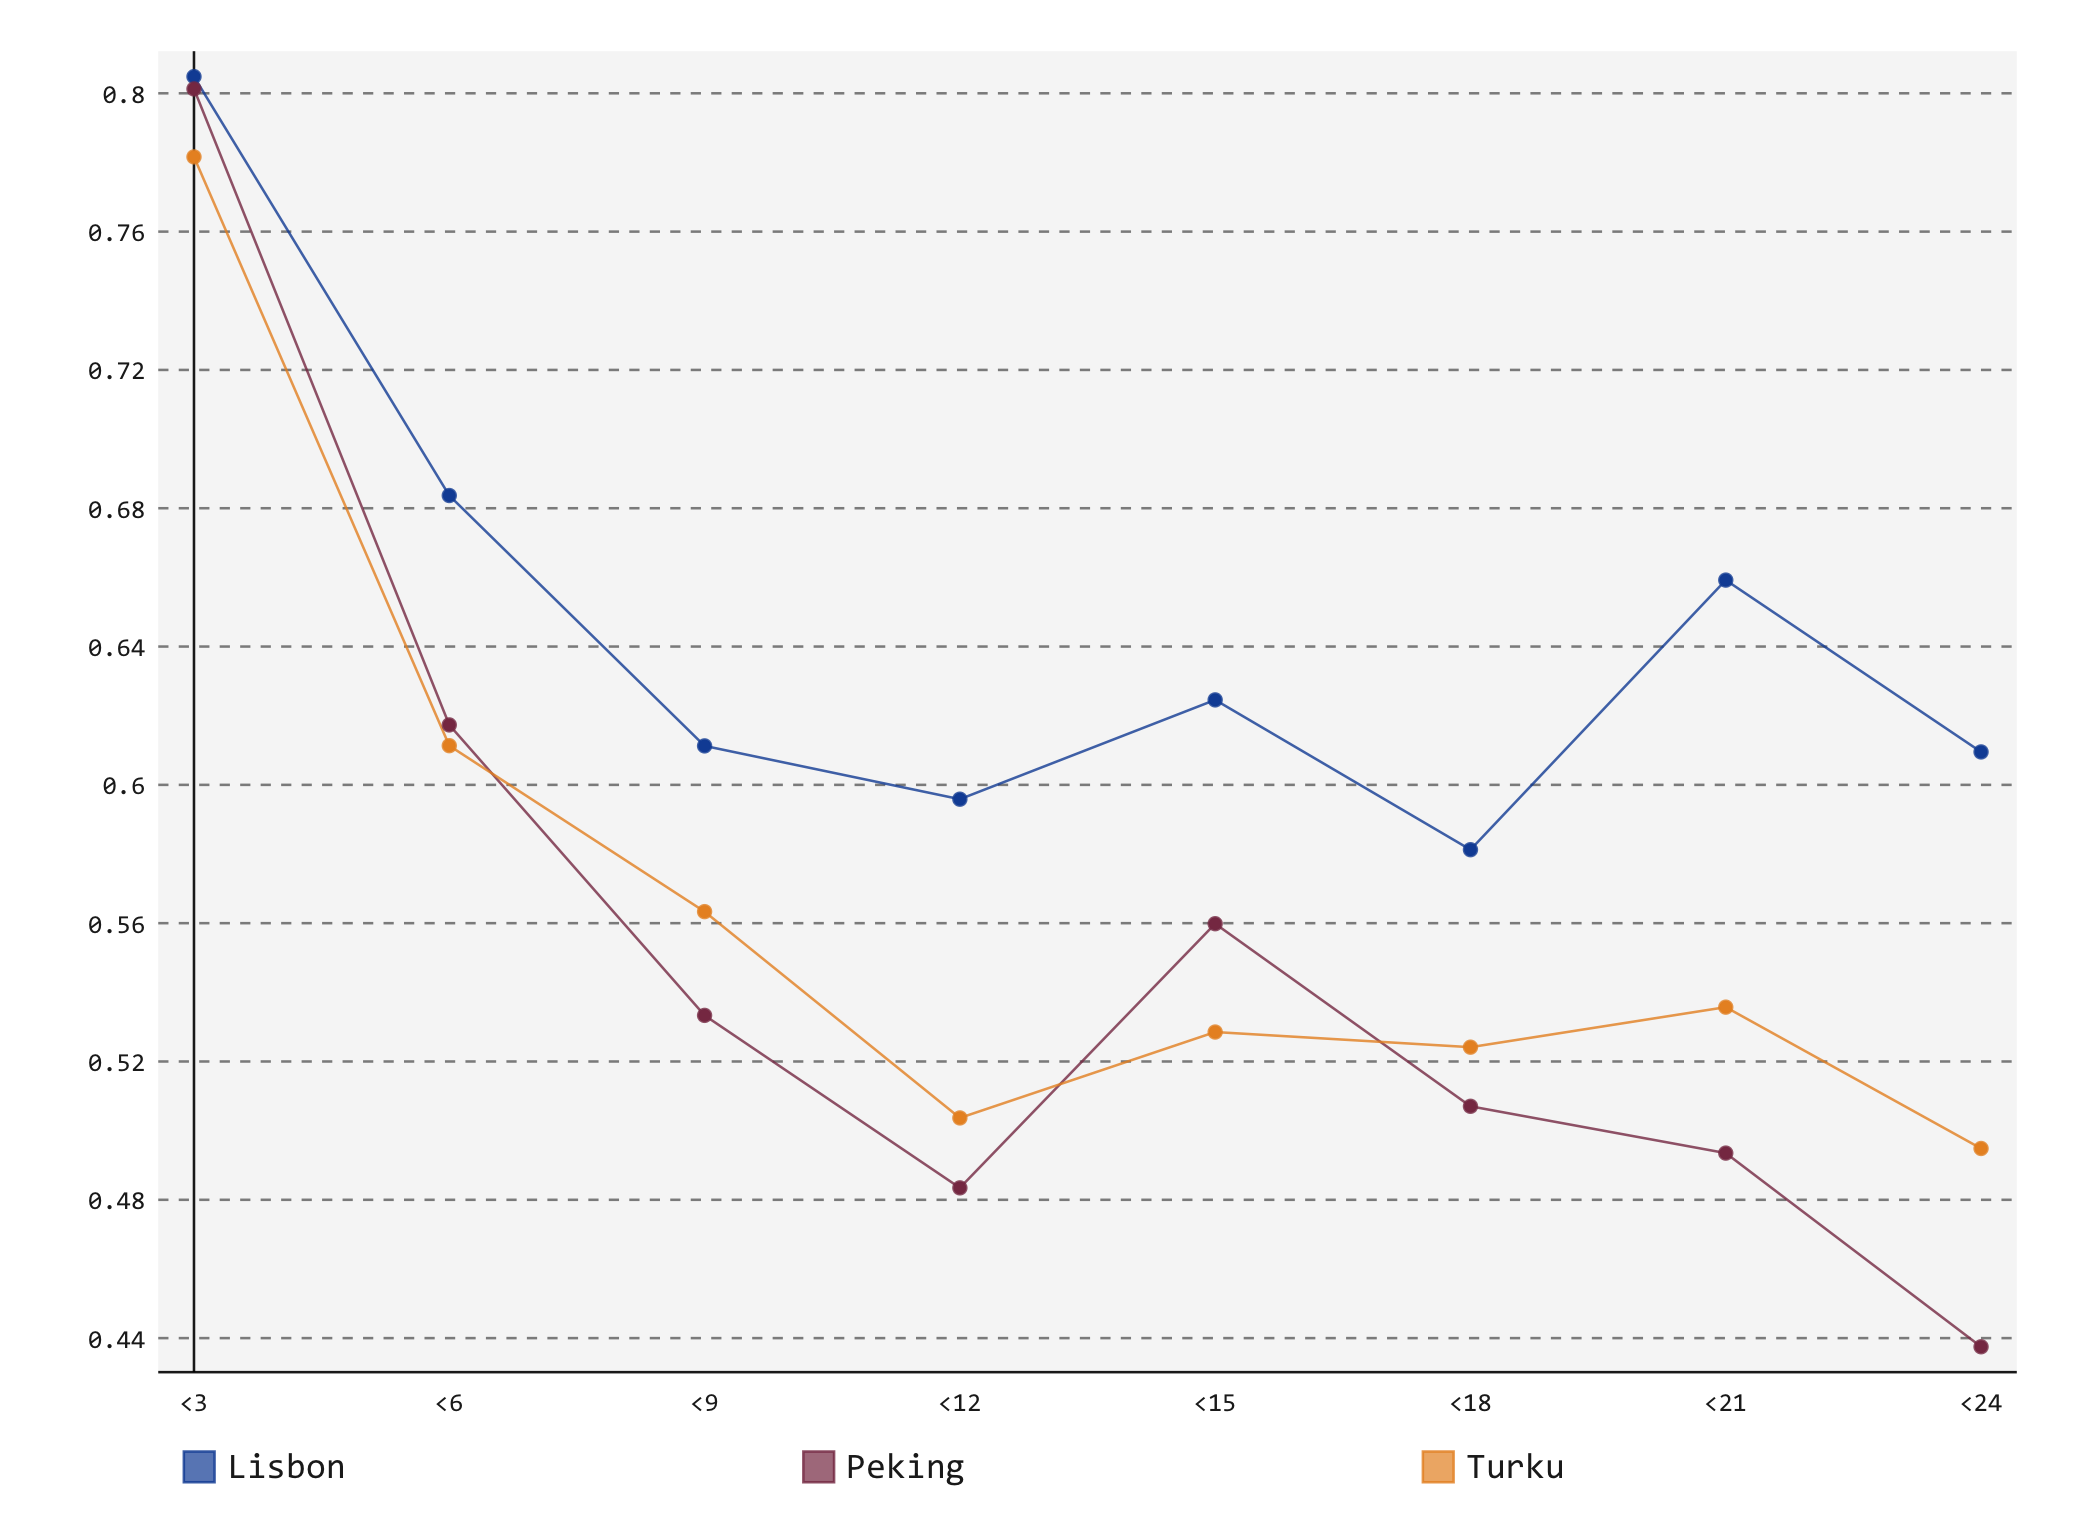
\includegraphics[width=\textwidth]{dep_len_fscore_PSD}
    \end{minipage}
    \caption{F-score for the three parsing systems on the PSD target representations for dependency length in bins of 3.}
    \label{fig:dep_len_fscore_PSD}
\end{figure}

\begin{table}
    \centering
    \smaller[0.5]
    \begin{tabular}{@{}lllllll@{}}
        \toprule
        \textbf{ } & \textbf{Gold} & \textbf{Test} & \textbf{Match} & \textbf{Precision} & \textbf{Recall} & \textbf{F-score} \\
        \midrule
        Peking &7678       &7681       &7406       & 96.42     & 96.46     & \textbf{96.44}    \\
        Lisbon &7678       &7727       &7425       & 96.09     & 96.70     & 96.40    \\
        Turku &7678       &7850       &7371       & 93.90    & 96.00     & 94.94    \\
        \midrule
        Peking &11600      &11736      &11508      & 98.06     & 99.21     & \textbf{98.63}    \\
        Lisbon &11600      &11912      &11494      & 96.49     & 99.09     & 97.77    \\
        Turku &11600      &12173      &11474      & 94.26     & 98.91     & 96.53    \\
        \bottomrule
    \end{tabular}
    \caption{Results for singletons on the DM (top) and PSD (bottom) target representations.}
    \label{fig:singletons}
\end{table}

\begin{figure}[h]
    \centering
    \begin{minipage}{0.8\textwidth}
        \centering
        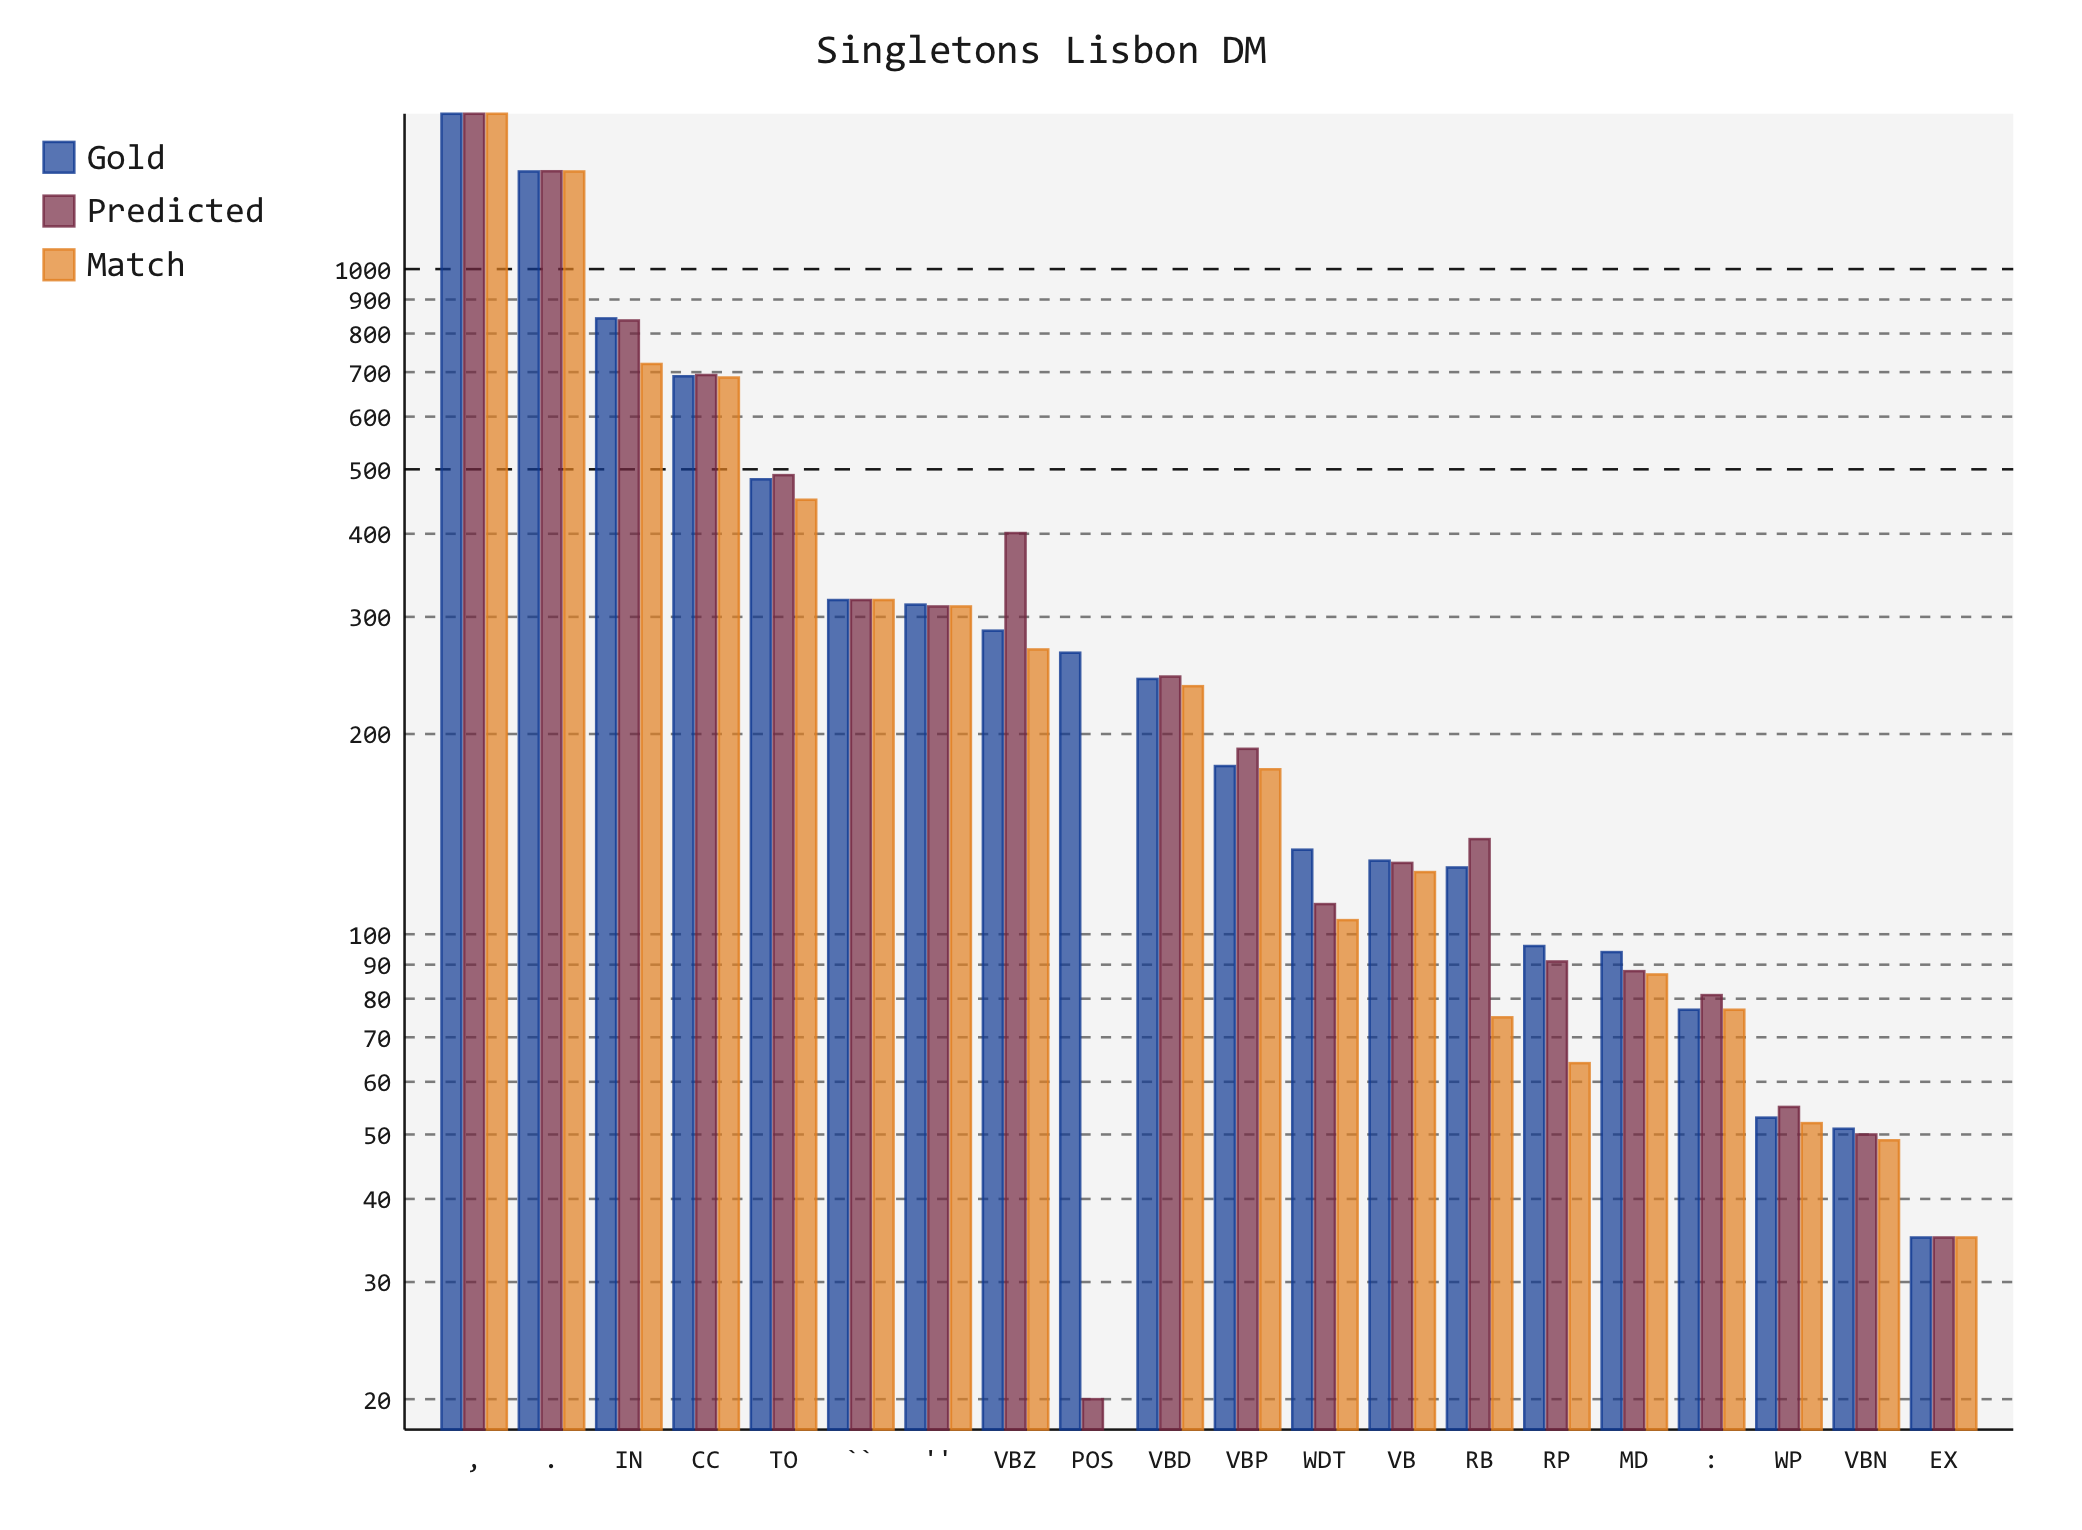
\includegraphics[width=\textwidth]{singletons_pos_DM}
    \end{minipage}\hfill
    \caption{Singletons broken down by punctuation and part-of-speech tags for the DM target representation for the Lisbon parsing system.}
    \label{fig:singletons_pos_DM}
\end{figure}

\begin{figure}[h]
    \centering
    \begin{minipage}{0.8\textwidth}
        \centering
        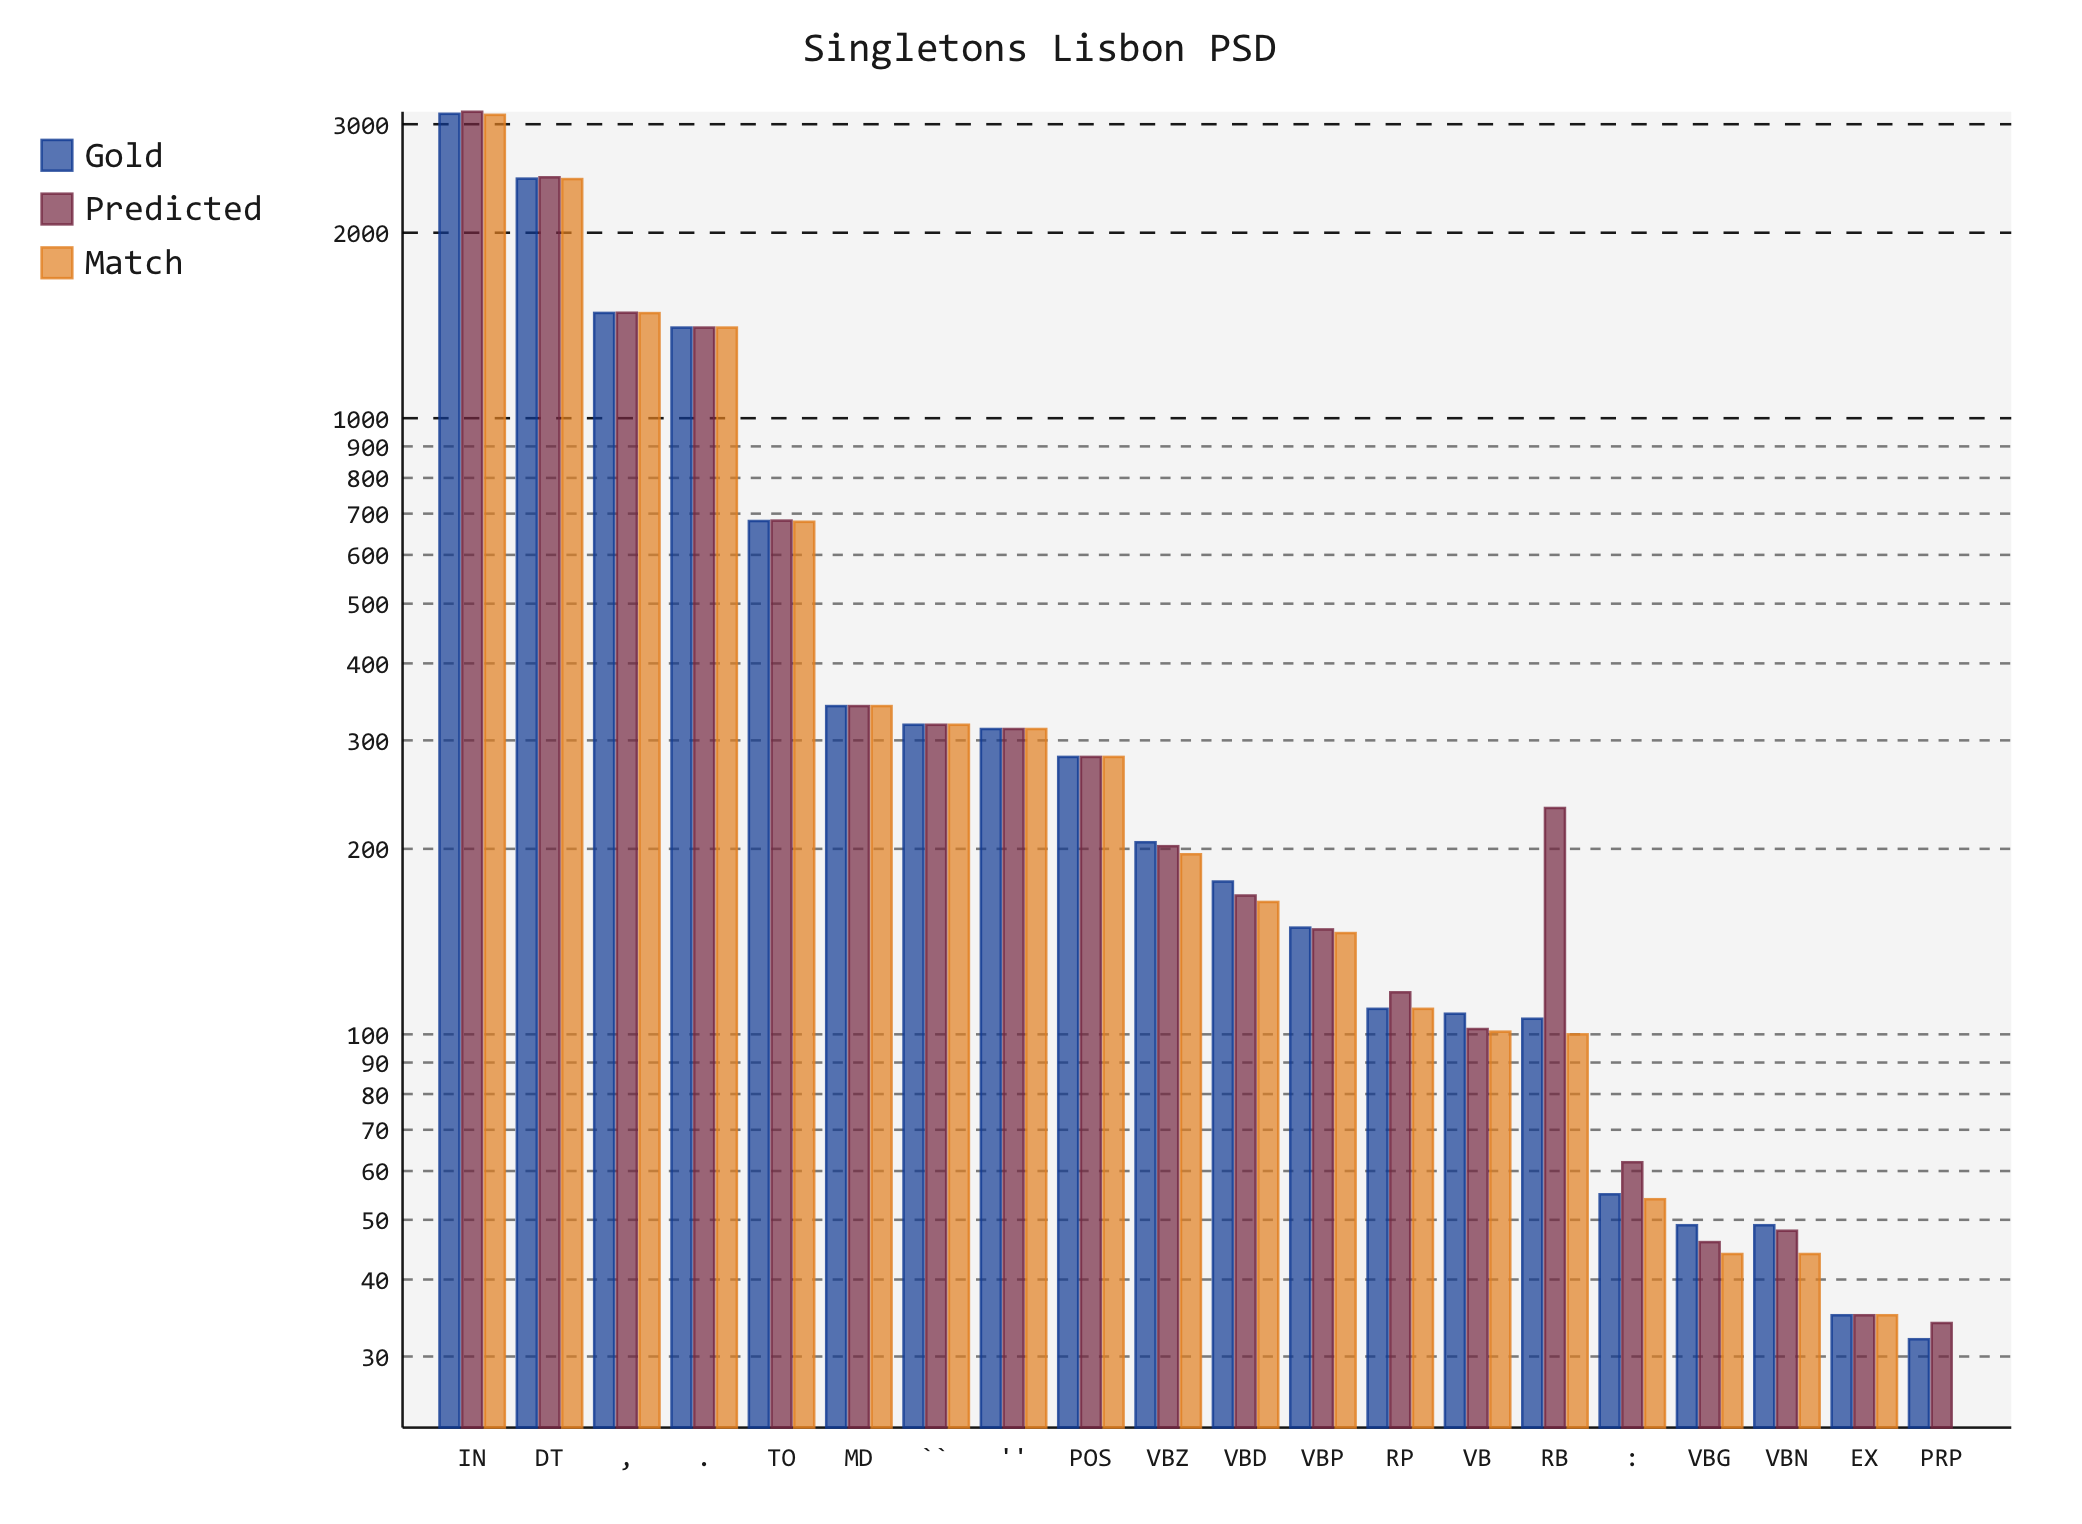
\includegraphics[width=\textwidth]{singletons_pos_PSD}
    \end{minipage}
    \caption{Singletons broken down by punctuation and part-of-speech tags for the PSD target representation for the Lisbon parsing system.}
    \label{fig:singletons_pos_PSD}
\end{figure}

\begin{figure}[h]
    \centering
    \begin{minipage}{0.8\textwidth}
        \centering
        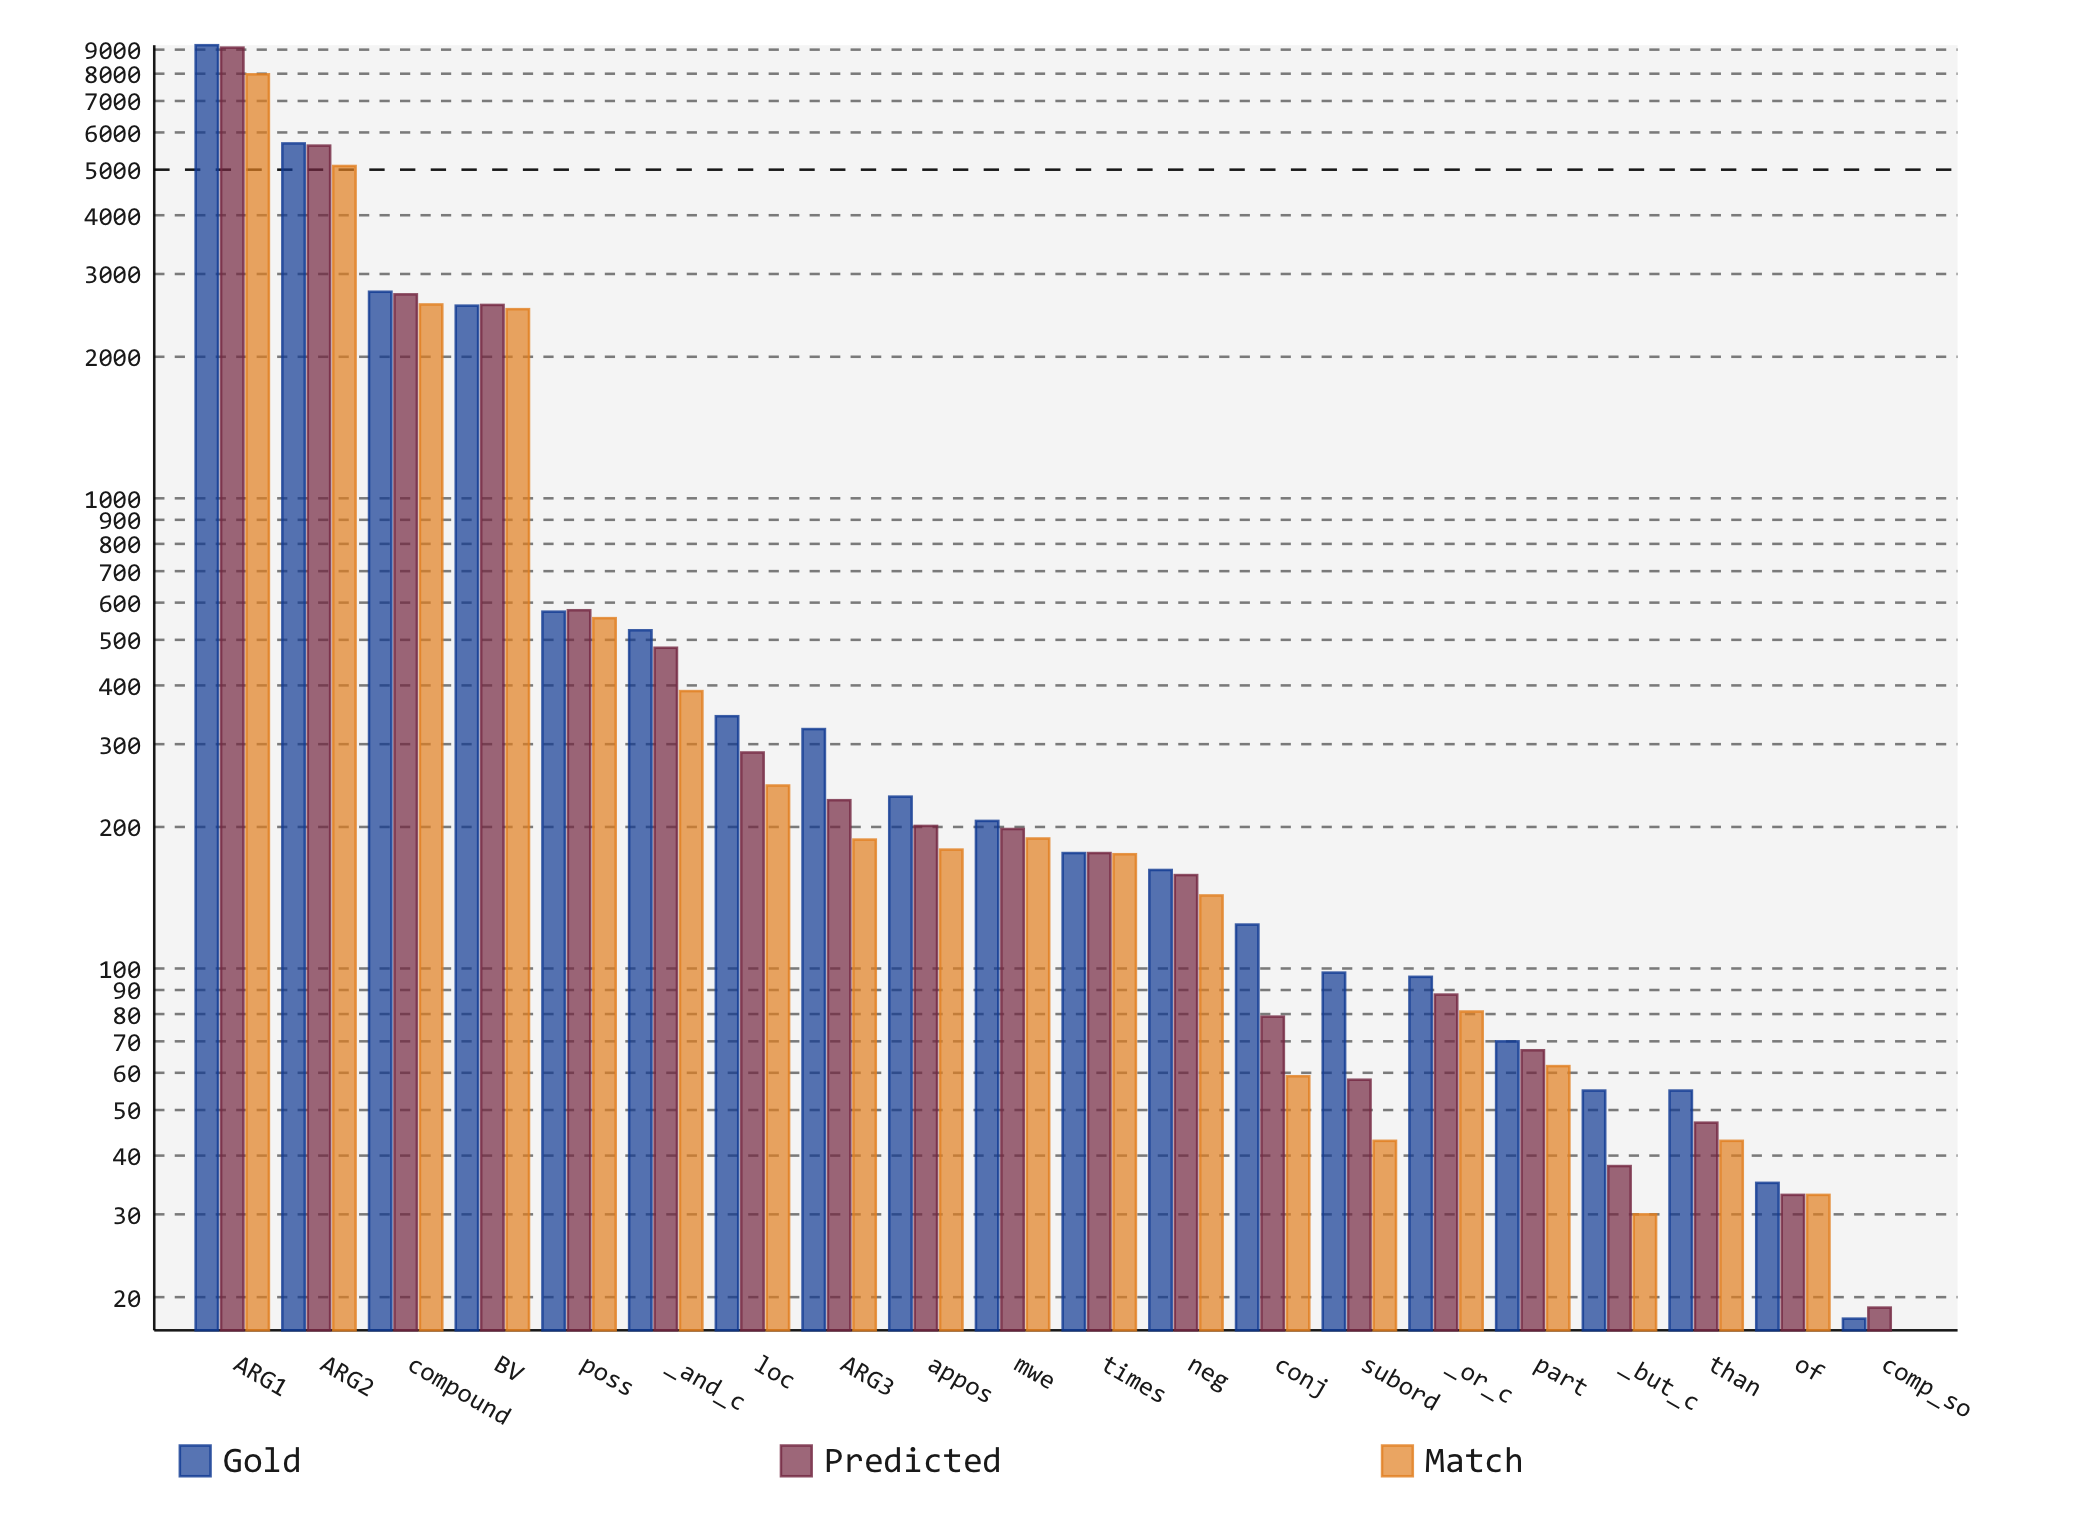
\includegraphics[width=\textwidth]{Lisbon_DM_Dep}
    \end{minipage}\hfill
    \caption{The 20 most frequent dependency types of the DM target representations. They numbers are for the frequency in gold data, the predicted data by the Lisbon parsing system, and the matches between the two.}
    \label{fig:lisbon_dep_DM}
\end{figure}

\begin{figure}[h]
    \centering
    \begin{minipage}{0.8\textwidth}
        \centering
        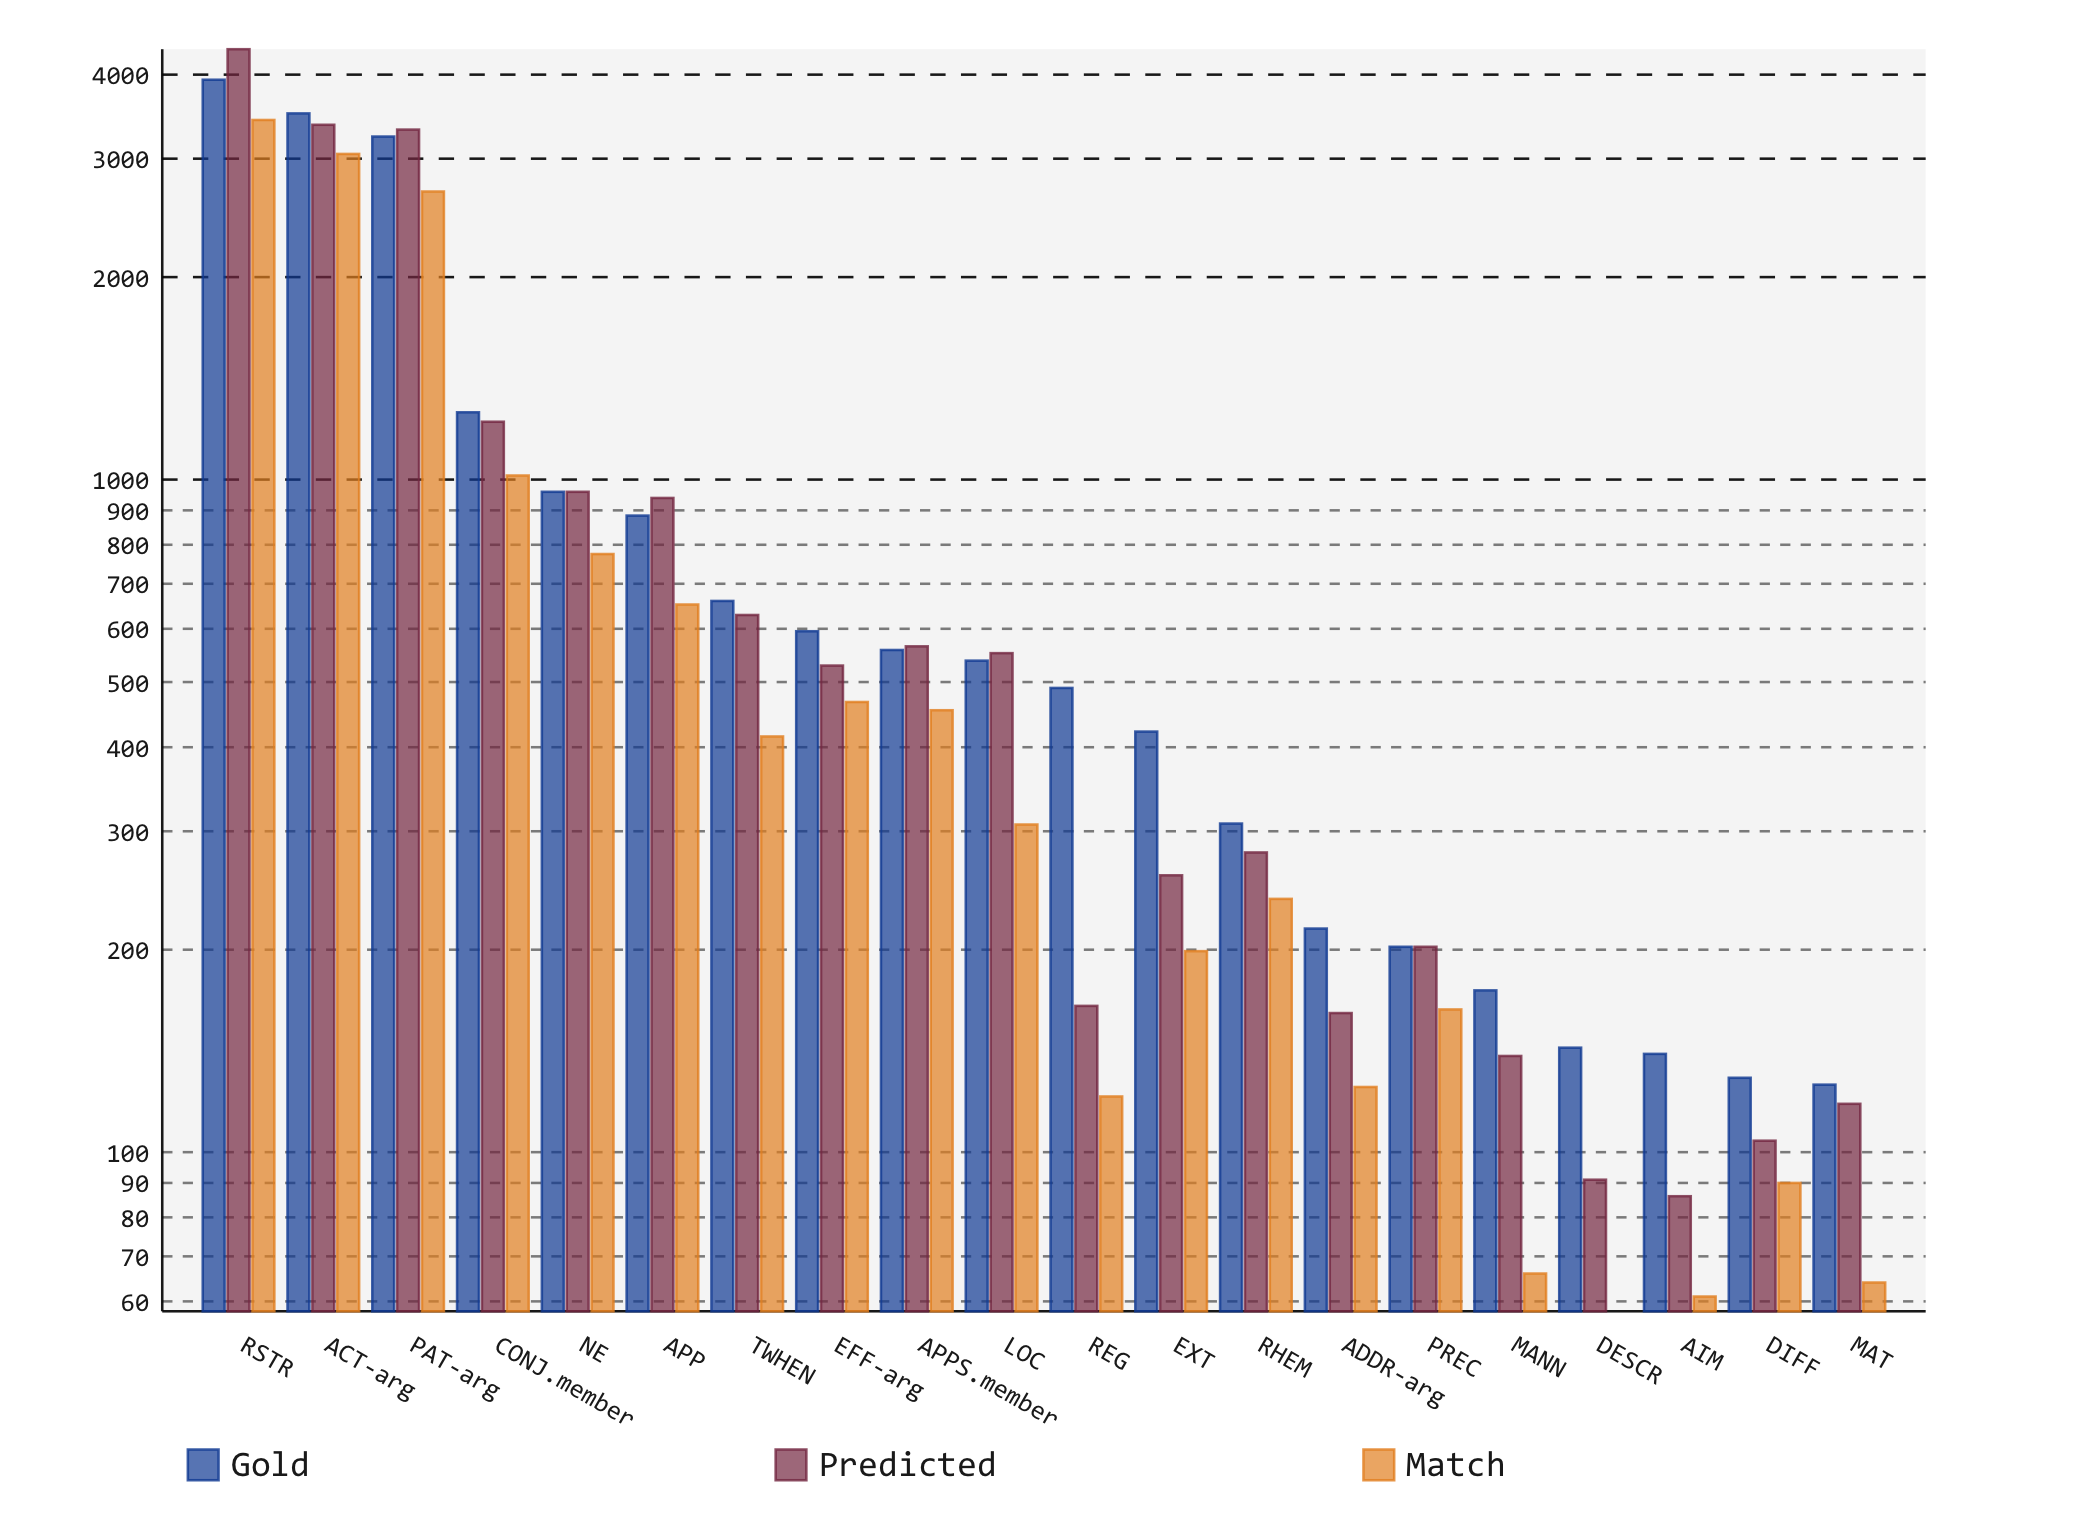
\includegraphics[width=\textwidth]{Lisbon_PSD_Dep}
    \end{minipage}
    \caption{The 20 most frequent dependency types of the PSD target representations. They numbers are for the frequency in gold data, the predicted data by the Lisbon parsing system, and the matches between the two.}
    \label{fig:lisbon_dep_PSD}
\end{figure}

\begin{figure}[h]
    \centering
    \begin{minipage}{0.8\textwidth}
        \centering
        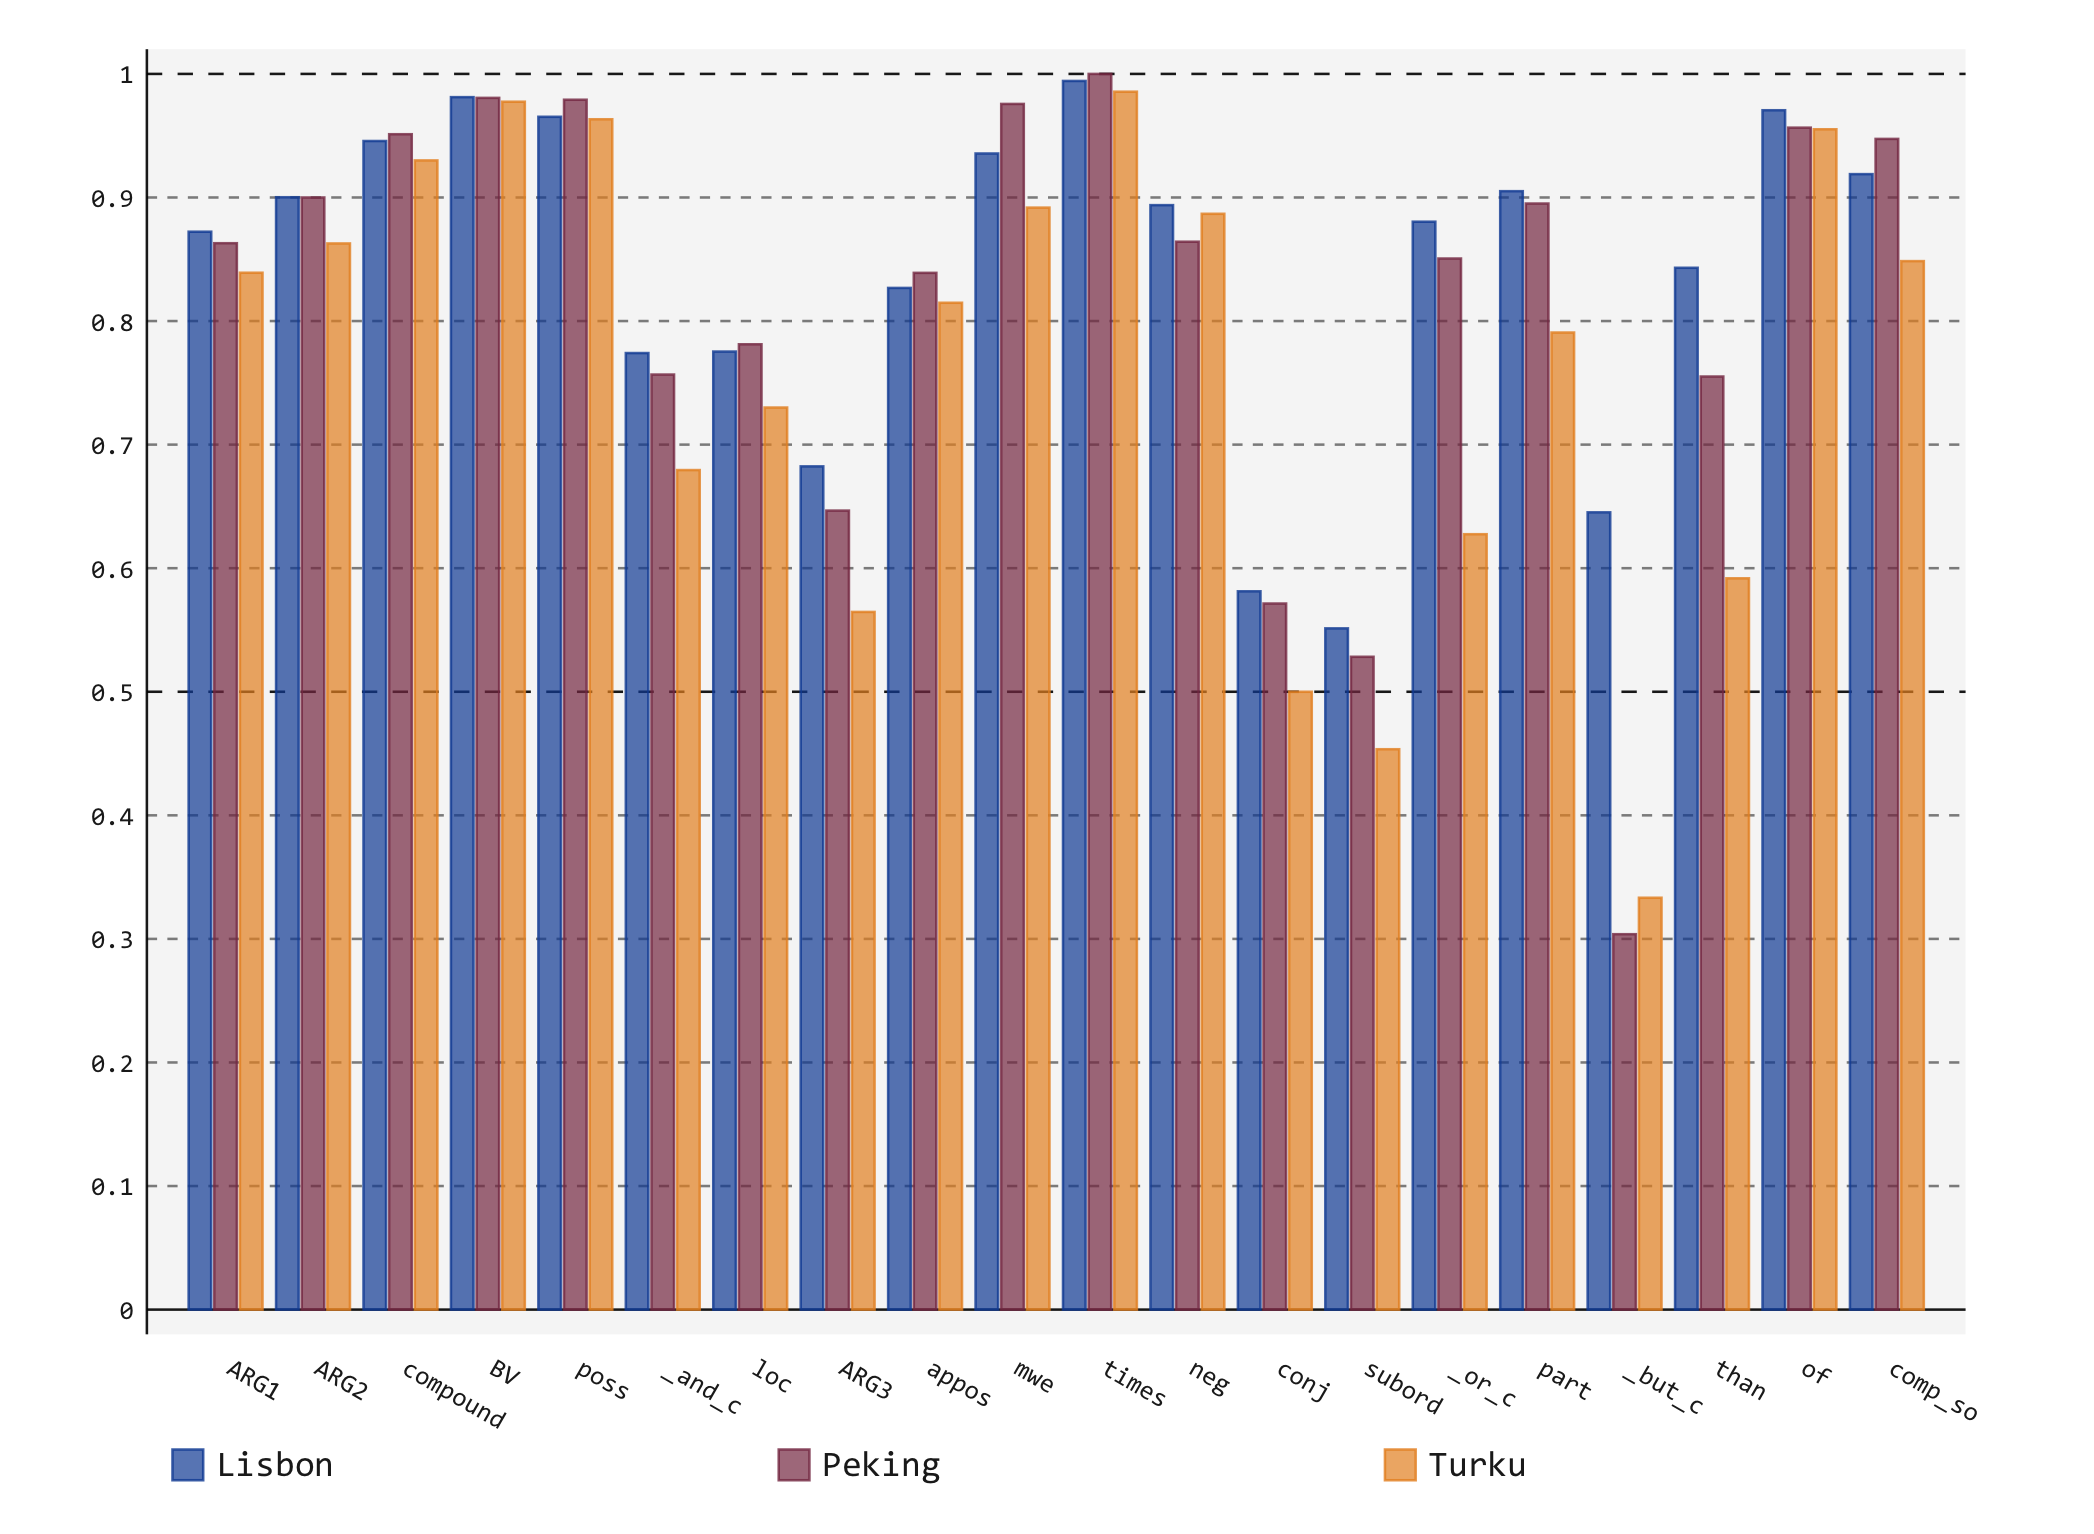
\includegraphics[width=\textwidth]{dep_dm_fscore}
    \end{minipage}\hfill
    \caption{F-score for the three parsing systems for the 20 most frequent dependency types for the DM target representations.}
    \label{fig:dep_fscore_DM}
\end{figure}

\begin{figure}[h]
    \centering
    \begin{minipage}{0.8\textwidth}
        \centering
        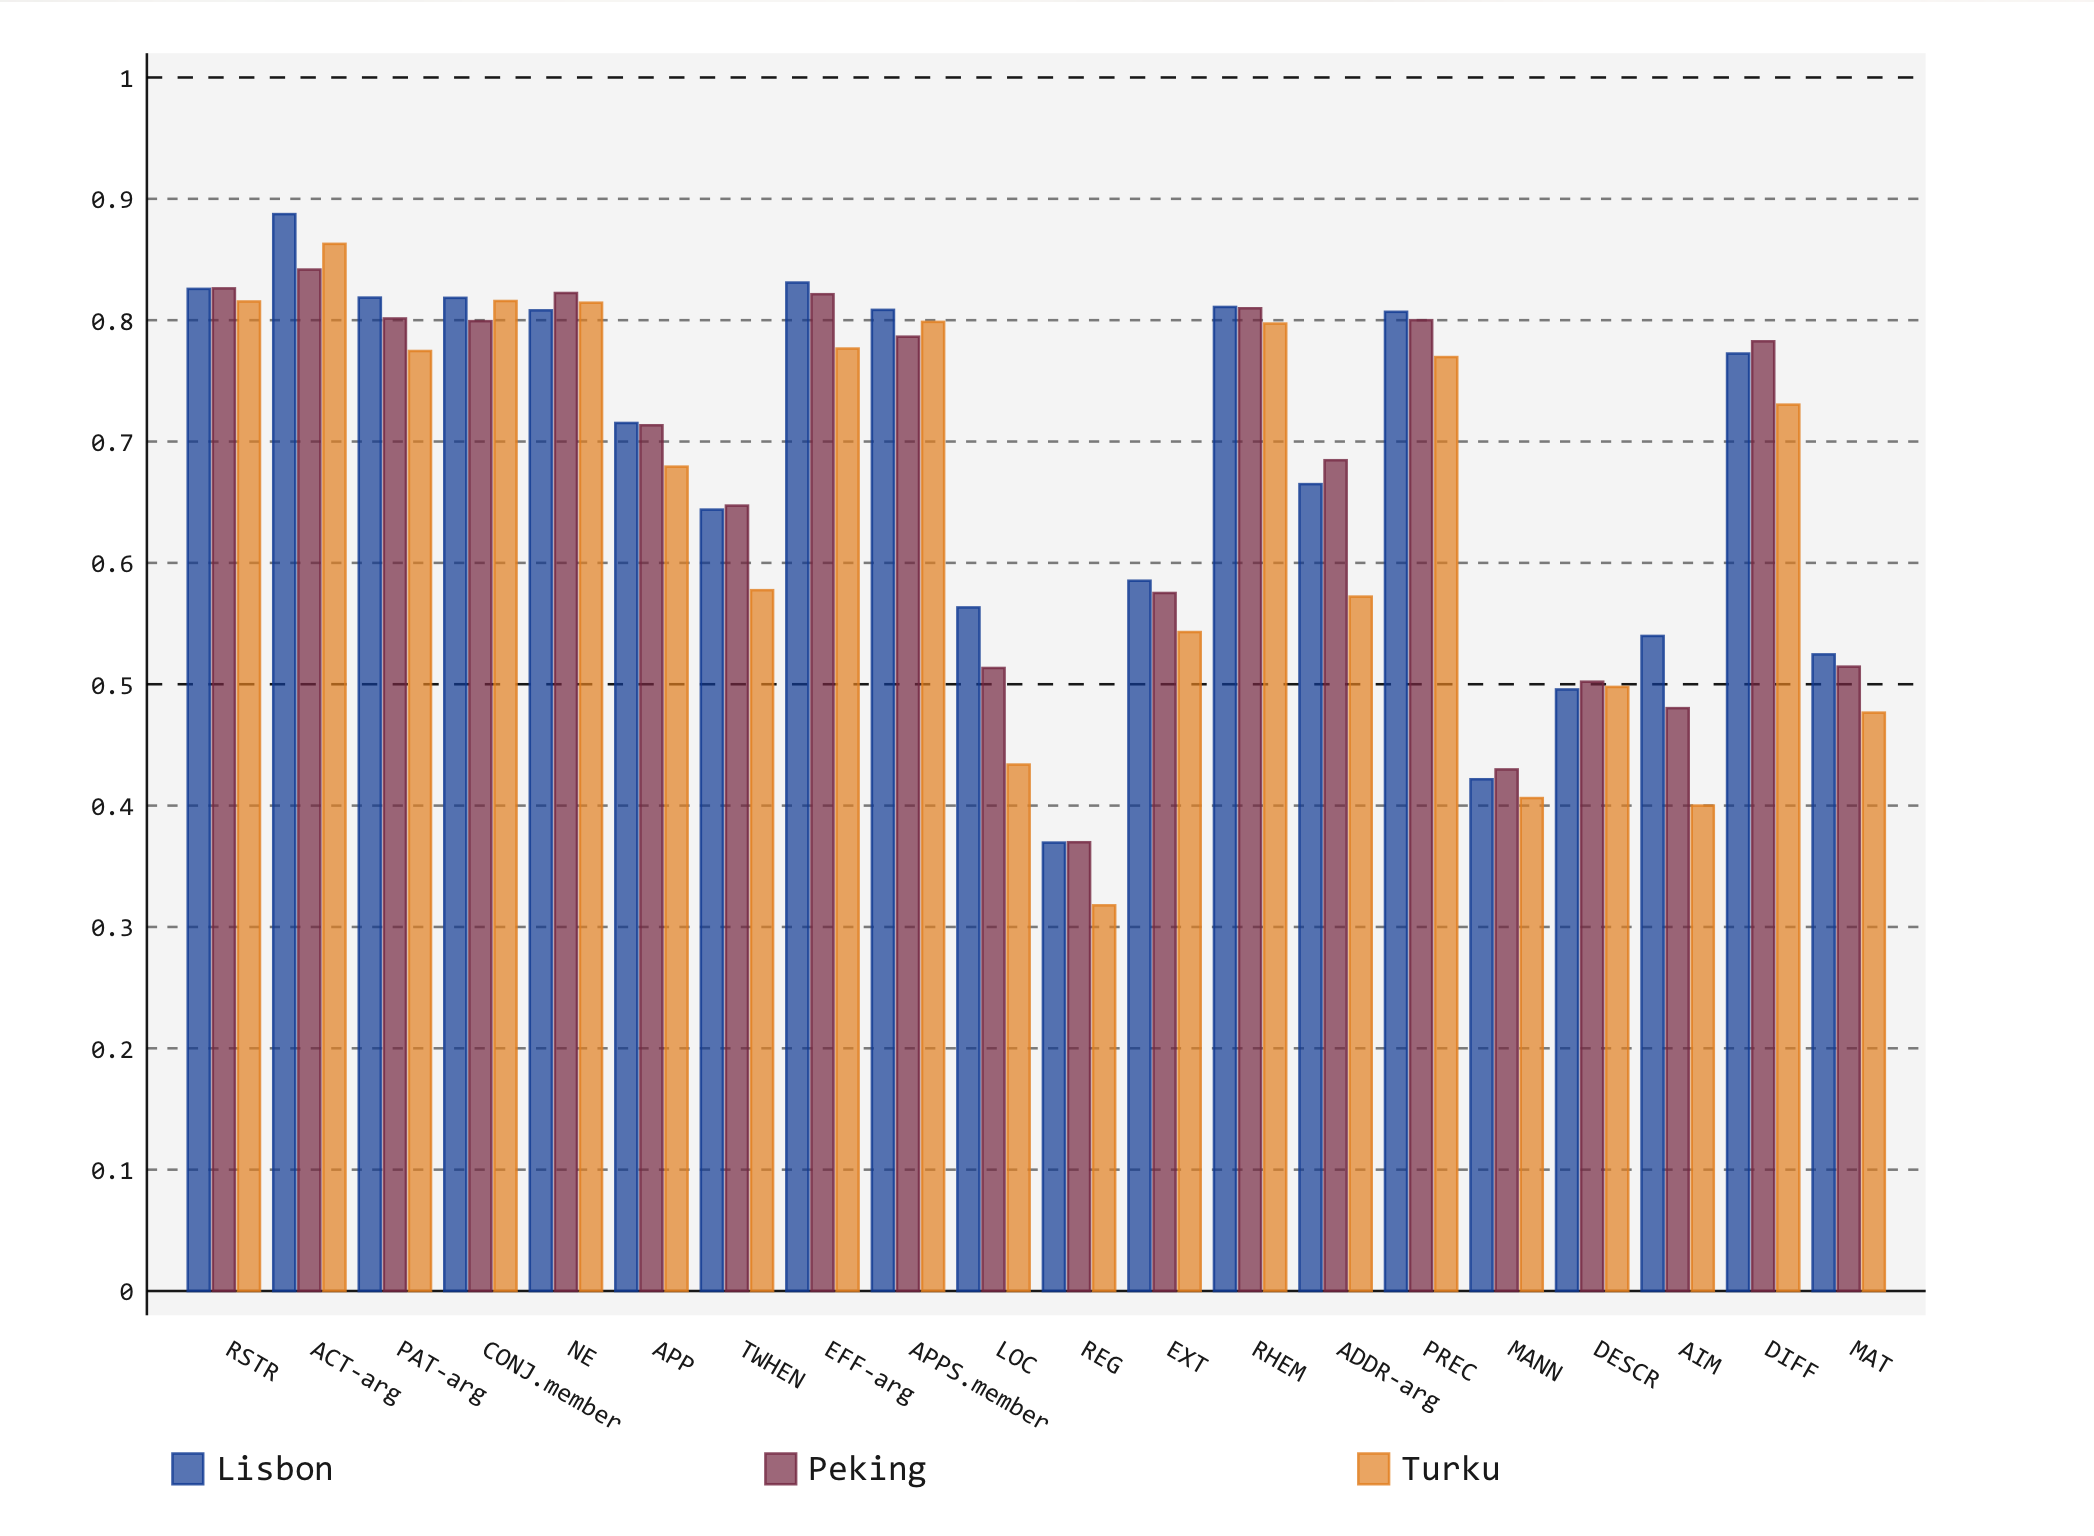
\includegraphics[width=\textwidth]{dep_psd_fscore}
    \end{minipage}
    \caption{F-score for the three parsing systems for the 20 most frequent dependency types for the PSD target representations.}
    \label{fig:dep_fscore_PSD}
\end{figure}

Another interesting phenomena is the accuracy of a parsing system relative to the length of dependencies. The parsing systems we examine have lower accuracy for longer dependencies. This is due to several reasons. One reason is sparsity, there are fewer longer dependencies than shorter. Another reason is that longer dependencies often represent more complex linguistic phenomena.

Observing the graphs in Figure \ref{fig:Lisbon_dep_len_DM}, \ref{fig:Lisbon_dep_len_PSD}, we see two graphs representing the number of dependencies of each length for the Lisbon parsing system. The graphs have a distribution over the dependencies in the gold data, the predicted dependencies, and the matches between the gold and predicted data (the correct predictions by the parser).

The most obvious observation observation is that the Lisbon parsing system makes fewer predictions than what is found in the gold standard data set on both the DM and PSD target representations. The exception occurs when dealing with shorter dependencies, and examining dependencies of length 1 (a dependency between adjacent words), we observe that there are more dependencies in the predictions than gold standard data on both DM and PSD. As the length of dependencies increase, the number of predictions and matches decrease. These same observations hold for the Peking and Turku parsing systems.

To further elaborate on this point, we introduce the F-score of all parsing systems in relation to dependency length in Table \ref{fig:dep_len_fscore_DM} and \ref{fig:dep_len_fscore_PSD} for both target systems. Here we have divided dependency length in bins of 3 in order to make the graphs more readable. The f-score of the parsing systems for dependency length show a substantial decrease as dependency lengths increase.

The performance of Lisbon is noteworthy in this regard, and this may be part of the explanation as to why its overall performance is better than Peking and Turku. The Lisbon systems has a substantially higher f-scores for longer dependencies. Peking and Turku have somewhat similar results, with Peking having higher f-score when dependency lengths are between 1 and 12, but lower for dependencies above 12 (overall). This might be explained by the fact that Turku participated in the open track, and thus had access to other resources such as a syntactic parser. It might also be due to technical details of the parsing systems.

All three parsing systems demonstrate a decline in f-score as dependency lengths increase on both the DM and PSD target representations. However, there is a slight return to higher f-scores once the dependencies reach lengths ranging from 12 to 18. This is most prevalent for the Lisbon parser, but is also observed in the Turku and Peking parsing systems.

% conclusion
Both sentence and dependency length have a distribution in the data sets where the frequency of a length factor is correlated with the accuracy for parsing that specific length. Overall we can state that the higher the frequency of a given length factor, the more likely it is that the parsing system has a higher accuracy when parsing a sentence or dependency with a given length. It is therefore important not to exaggerate the importance of the length factor itself, but also take into account the distribution with which it occurs in the data used for training and testing. A different data set and distribution would result in, if our assumptions are correct, parsing systems with a different correlation between length and accuracy.

However, since we are dealing with natural language, we can also assume that a relatively similar distribution of sentence and dependency lengths observed in the SemEval-2015 data sets will be prevalent in other corpora. It is therefore important for any research on dependency parsing to consider length factors, and experiment with various methods to deal with the particular aspects of sentence and dependency length that might impact accuracy.

It is also important not to fully downplay the linguistic factors that may impact the accuracy in relation to the length factors. Longer sentences include more complex sentence structure, and longer dependencies include more complex grammatical structures.

We will now turn our attention to specific graph factors: singletons, and examine the accuracy of the three parsing systems in relation to these aspects of semantic dependency parsing.













\section{Graph factors}
% projectivity
% singletons

As for graph factors we will examine the accuracy of the parsing systems of our analysis in relation to singletons, i.e. nodes that have been left outside of the dependency graph. This factor is specific to semantic dependency parsing, as with syntactic dependency parsing all lexical units are connected. In the semantic dependency graphs of the DM and PSD target representations, so-called semantically vacuous lexical units are left outside the dependency graph. We will examine how the three parsing systems perform in accurately predicting these.

\subsection{Singletons}

Examining Table \ref{fig:singletons}, we can see the results of the three parsing systems in accurately predicting singletons. To be precise, the prediction of singletons in the three parsing systems are the result of nodes left out from the dependency structure rather than being part of a classification task. This is a step that could be considered as a binary classification task in its own right. However, the three parsing systems that we examine do not make any explicit classification of singletons, and the nodes left outside the graph are a side-effect of the parsing.

Looking closer at Figure \ref{fig:singletons}, we see that for the both target representation, Turku is the parser that has the highest number of singletons as the byproduct of its parsing, but a large portion of these should in fact be part of the dependency structure. The other two parsing systems also have a higher number of singletons than the gold standard. All parsing systems could therefore increase the accuracy of their parsing by attempting to parse more lexical units as part of the dependency structure. However, the accuracy in relation to singletons is relatively high.

A few cases do stand out when it comes to singletons. Examining Graphs \ref{fig:singletons_pos_DM} and \ref{fig:singletons_pos_PSD}, we observe that for certain part of speech tags, the accuracy is quite dramatically different than the others. In DM this is the case for `VBZ' (verb, 3rd person singular present), `VBD' (verb, past tense), `POS' (possessive ending), `RP` (particle) and `RB' (adverb) tags. For the PSD target representation the `RB' (adverb) tag stand out. 

It is not clear as to why certain type of singletons are more difficult to parse than others. Classifying singletons could be seen as a distinct binary classification task. Pursuing this task one could examine closely the specific type of singletons that are problematic for the parsing systems we are examining. A singleton classifier could then possibly be used as a pre-processing step before parsing, or as a post-processing step to clean up possible errors of the parsing systems. However, since we have decided to pursue the task of semantic frame classification, we leave this task open.

% As we can see from Table \ref{fig:singletons}, the precision and recall of the Lisbon parsing system for the PSD target representation is quite higher than for DM.








\section{Linguistic factors}
% part of speech
% labels

The linguistic aspects of semantic dependency parsing that we will include in this analysis are dependency types. When dealing with dependency types, the analysis will differ to a higher degree between the target representations than other factors. This is due to the fact that annotation schemes used in different target representations can be based on very different set of labels. It is therefore important to note that the analysis in this section may not be as general as our other findings such as the length factors.

\subsection{Dependency types}

The dependency types found in the DM and PSD target representations follow different annotations schemes. This is true for both the number of dependencies, their distribution and what they signify. In the test data set, the DM target representation has 43 dependency types and 24813 dependencies, whereas the PSD target representation has 77 types and 22258 dependencies.

If we examine Figures \ref{fig:lisbon_dep_DM} and \ref{fig:lisbon_dep_PSD}, we have two graphs of the 20 most frequent dependency types for both the DM and PSD target representation. The graphs present the number of dependencies in the gold data, the predictions made by the Lisbon parser, and the number of matches between the predicted and gold. We see that for the DM target representation the first two dependency types, `ARG1' and `ARG2', account for 14884 of the 24813 dependencies, while for the PSD target representation the distribution is more evenly spread across the most frequent types. In terms of the parsing accuracy, we see that the number of gold and predicted dependencies are more similar for DM than for PSD, where there are more fluctuations.

From the two Figures \ref{fig:lisbon_dep_DM} and \ref{fig:lisbon_dep_PSD}, we observe that the parsing of the Lisbon parser is relatively conservative, i.e. there are less dependencies in the output than there are in the gold standard data. This is particularly evident for dependencies that are less frequent.

As we observed with singletons, there are a few dependency types that stand out with a larger margin of error. Examining Figure \ref{fig:lisbon_dep_DM} we see that for Lisbon on the DM target representation there is a great mismatch between the number of frames in the gold data, the predicted dependencies, and the match, for certain type of dependencies such as `conj' (conjunction) and `subord' (subordination). These are more complex grammatical structures than for instance `ARG1' and `ARG2'.

In Figures \ref{fig:dep_fscore_DM} and \ref{fig:dep_fscore_PSD} we see the f-scores of our parsers over the same distribution of the top 20 most frequent dependencies. There is a large discrepancy between the three parsers for each dependency type, indicating that the technical differences play a role in this regard. The differences are less pronounced for the most frequent dependency types, but for `\_and\_c', `ARG3', `\_or\_c', `part', and `\_but\_c', the variations are substantial. Although less extreme, we see the same tendencies for the PSD target representation. This indicates that the errors that the three parsing systems of this analysis make are closely related to their underlying algorithms. 

An ensemble method of the semantic dependency parsing systems of our analysis might be an interesting approach if one is able to exploit the relative strengths of each system. An approach could be to take the output of all three parsers and by way of some heuristics choose the most probably dependencies based on the information of their respective error rates for each dependency type. 

However, we would still face low scores for the type of dependencies where all three parsing systems have a low f-score. We also observe that for the most part, the Lisbon parser has a higher f-score on the individual dependency types, so with an ensemble method we would only boost the scores of those dependency types where the other parsers have a higher score.

We now turn to the last aspect of semantic frames as the last part of our contrastive analysis. We will show that in relation to the other factors that we have examined in this chapter, semantic frames looks like the most promising for improvements.


















\section{Semantic Frames}

\begin{figure}[h]
    \centering
    \begin{minipage}{0.8\textwidth}
        \centering
        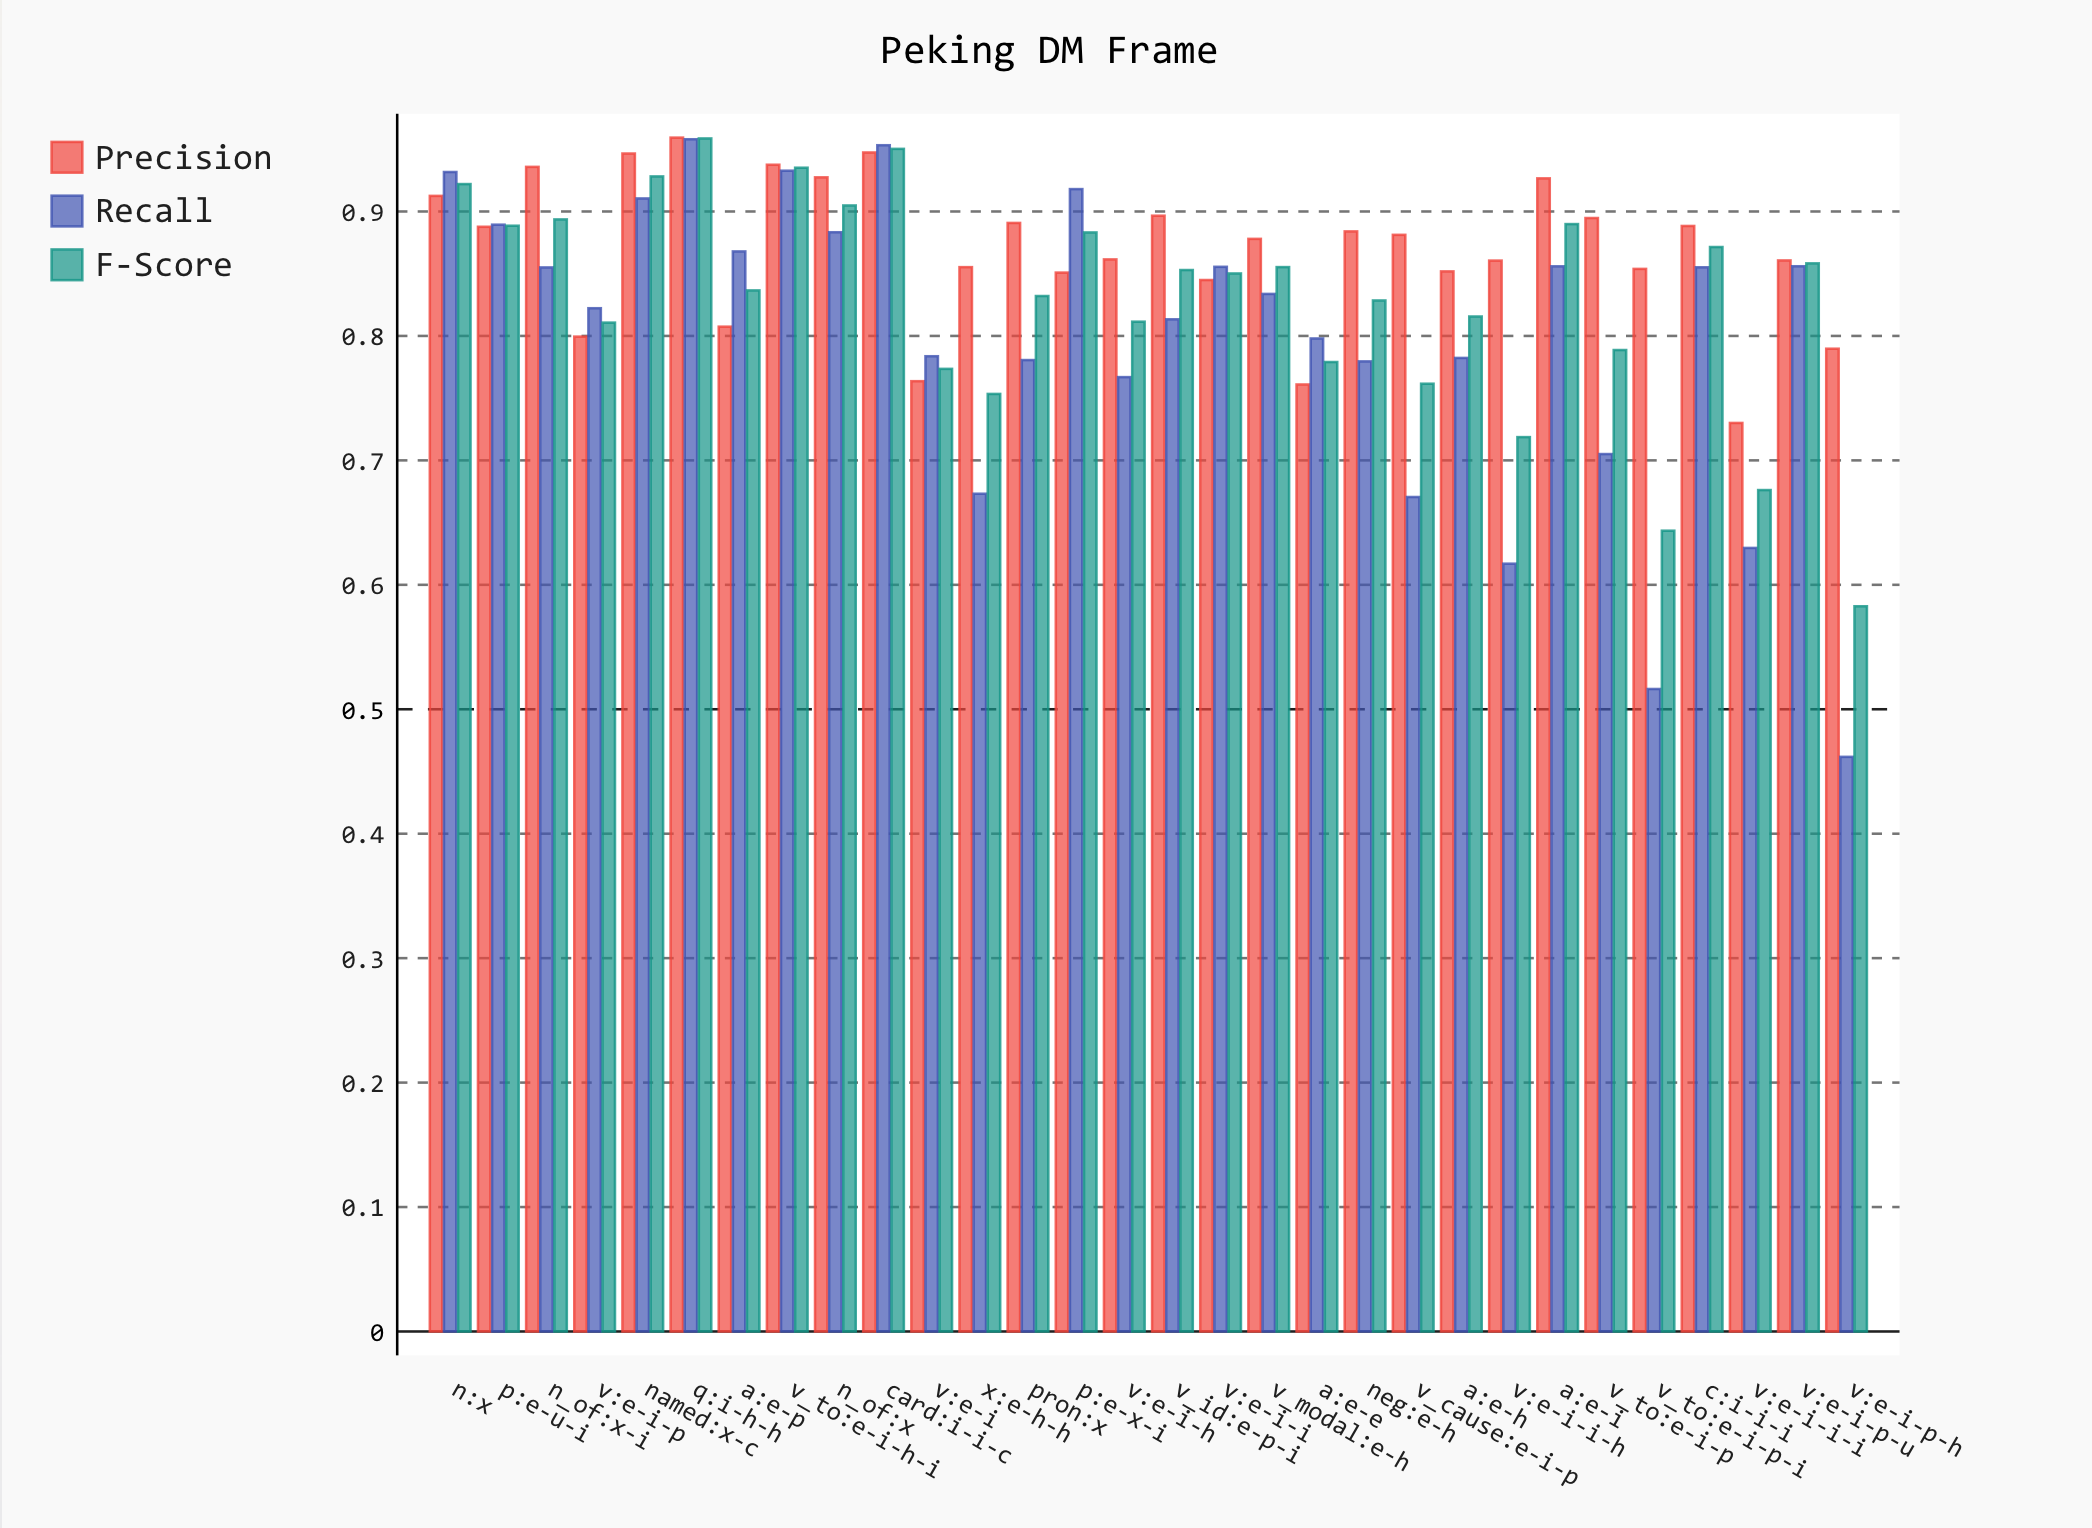
\includegraphics[width=\textwidth]{Peking_DM_frames_prf}
    \end{minipage}
    \caption{Precision, recall and f-score for of frames for Peking}
    \label{fig:Peking_frame_prf}
\end{figure}

\begin{figure}[h]
    \centering
    \begin{minipage}{0.8\textwidth}
        \centering
        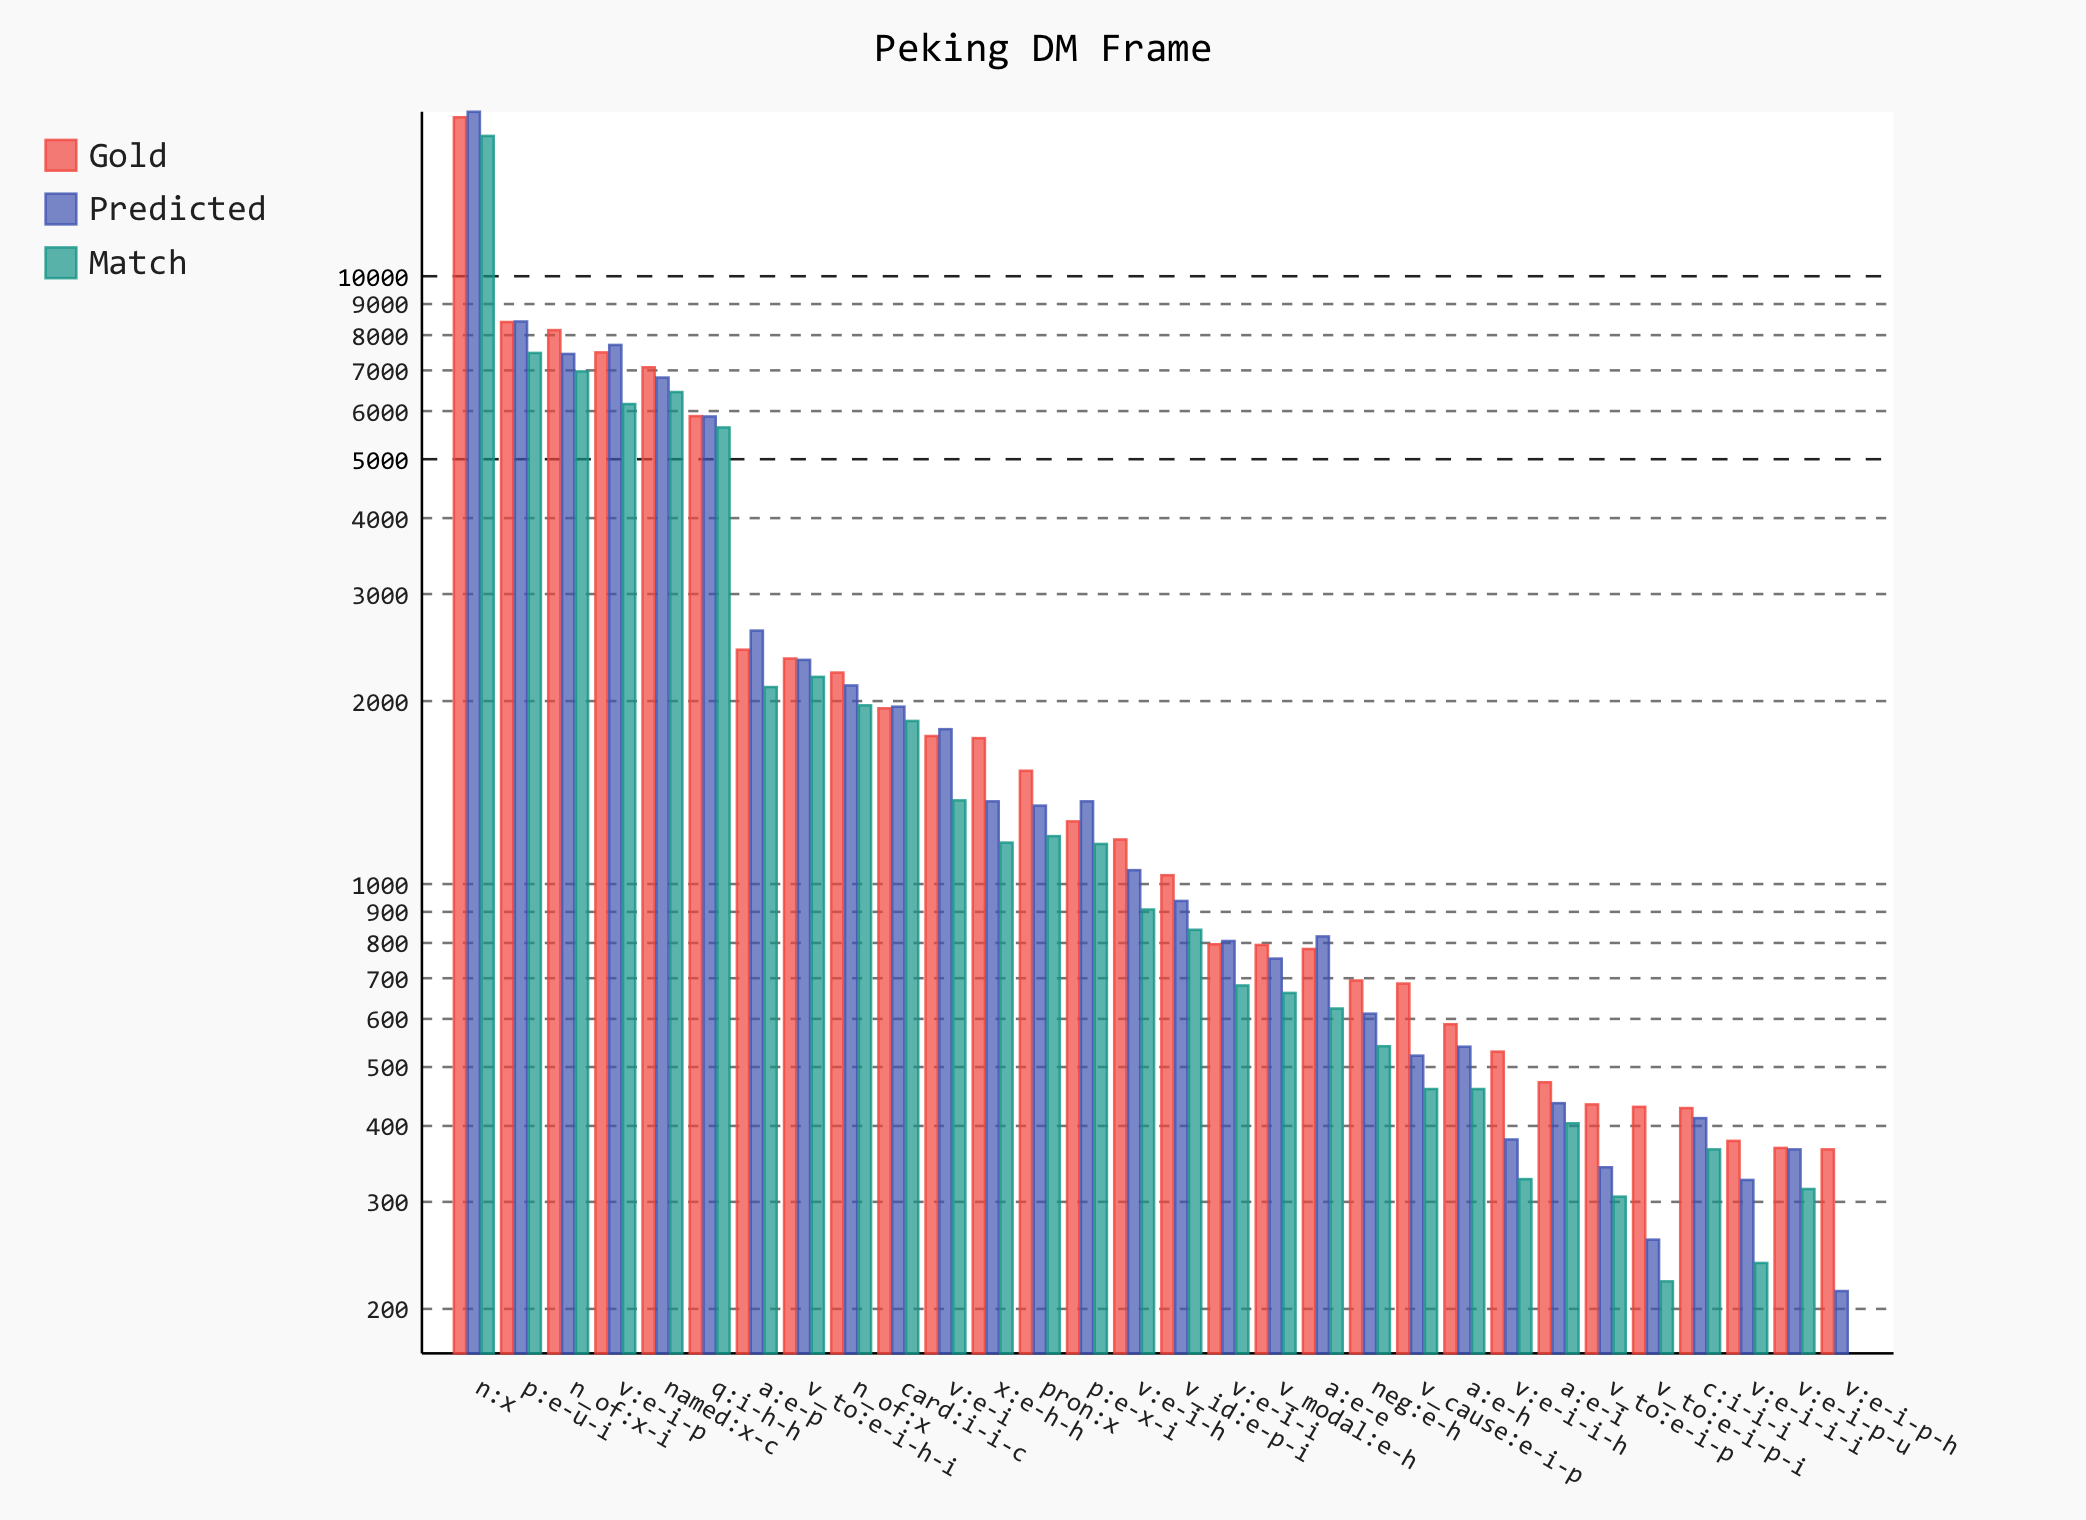
\includegraphics[width=\textwidth]{Peking_DM_frames}
    \end{minipage}
    \caption{The distribution of the 30 most frequent frames for Peking. The numbers are for gold standard frames, predicted frames by the Peking parsing system, and the correct matches.}
    \label{fig:Peking_frame_30}
\end{figure}

\begin{table}
    \centering
    \smaller[0.4]
    \begin{tabular}{@{}llllll@{}}
        \toprule
        \textbf{Frame} & \textbf{Total} & \textbf{Percent} & \textbf{Frame*} & \textbf{Total*} & \textbf{Percent*} \\
        \midrule
        n:x & 115049 & 18.64 & n:x & 4529 & 18.69 \\
        q:i-h-h & 72278 & 11.71 & q:i-h-h & 2891 & 11.93 \\
        named:x-c & 62208 & 10.08 & named:x-c & 2549 & 10.52 \\
        p:e-u-i & 54513 & 8.83 & p:e-u-i & 2061 & 8.51 \\
        n\_of:x-i & 45542 & 7.38 & n\_of:x-i & 1614 & 6.66 \\
        v:e-i-p & 34475 & 5.59 & v:e-i-p & 1342 & 5.54 \\
        a:e-p & 27802 & 4.5 & a:e-p & 988 & 4.08 \\
        card:i-i-c & 27128 & 4.39 & card:i-i-c & 902 & 3.72 \\
        pron:x & 14187 & 2.3 & pron:x & 647 & 2.67 \\
        n\_of:x & 12701 & 2.06 & n\_of:x & 510 & 2.1 \\
        \midrule
        Total & 465883 & 75.48  & Total & 18033 & 74.43 \\
        \bottomrule
    \end{tabular}
    \caption{The frequency distribution of frames in the training and test id (marked *) id for the DM target representation.}
    \label{table:dm_frames_freq}
\end{table}

\begin{table}
    \centering
    \smaller[0.7]
    \begin{tabular}{@{}llllll@{}}
        \toprule
        \textbf{Frame} & \textbf{Total} & \textbf{Percent} & \textbf{Frame*} & \textbf{Total*} & \textbf{Percent*} \\
        \midrule
        ev-w218f2 & 8355 & 9.35 & ev-w218f2 & 374 & 10.18 \\
        ev-w2833f1 & 7482 & 8.37 & ev-w2833f1 & 350 & 9.53 \\
        ev-w1566f3 & 1731 & 1.94 & ev-w1566f3 & 74 & 2.01 \\
        ev-w1239f1 & 845 & 0.95 & ev-w2888f2 & 51 & 1.39 \\
        ev-w218f3 & 821 & 0.92 & ev-w218f3 & 38 & 1.03 \\
        ev-w2888f2 & 810 & 0.91 & ev-w410f1 & 31 & 0.84 \\
        ev-w2772f1 & 801 & 0.9 & ev-w2875f4 & 29 & 0.79 \\
        ev-w218f7 & 657 & 0.73 & ev-w1239f1 & 28 & 0.76 \\
        ev-w410f1 & 612 & 0.68 & ev-w2671f1 & 24 & 0.65 \\
        ev-w3525f6 & 567 & 0.63 & ev-w3586f1 & 22 & 0.6 \\
        \midrule
        Total & 22681 & 25.37  & Total & 1021 & 27.8 \\
        \bottomrule
    \end{tabular}
    \caption{The frequency distribution of frames in the training and test id (marked *) id for the PSD target representation.}
    \label{table:psd_frames_freq}
\end{table}

Similar to dependency types, there is also a high degree of difference between the two target representations that we are examining. Actually, for PAS, there are no semantic frames in the annotations.  In Table \ref{table:dm_frames_freq} and \ref{table:psd_frames_freq}, we see some statistics on the frames in the data sets. It is worth noting that we exclude a range of semantic frames in this study. This is done so that we may follow the scoring scheme set forth by the SemEval-2015 organizers, which the semantic frame scores for all the parsing systems are based upon.

The SemEval-2015 scoring scheme reduces the number of frames to be part of evaluation by only including frames for tokens that have a \textit{part of speech tag} that starts with the letter 'V'\footnote{Part of speech tags that are equal to `MD' should also have been included in this selection if the goal is to check for all possibly ambiguous verbs. Since we are interested in comparing our results to that of the SemEval-2015 submissions, we follow the scoring practices of the organizers.}, and are classified as being predicates\footnote{Some details on evaluation can be found here: \url{https://tinyurl.com/msh6jr8}. However, the specific details on the exclusion of frames not starting with `V' and being a predicate are not present in any of the scientific papers that we have examined. The scoring scheme was revealed by examining the scoring files included in the package with the training and testing data}, i.e. a node with outgoing dependency edges in the semantic dependency graph. This was done in order to only score frames on potentially ambiguous verbs.

Both the number of unique frames and instances in the data sets have been reduced substantially by the scoring scheme, and the number of frames in DM and PSD are closer to each other. The DM and PSD in-domain data have 3459 and 3584 instances of frames to classify respectively, and 3750 and 3919 on the out-of-domain test data respectively. This makes it possible to have a more empirically similar base for comparing the results when classifying semantic frames on both target representations. However, the number of unique frames are still somewhat skewed, where the unique number of frames in both training and testing are substantially higher for PSD in comparison to DM.

Examining Tables \ref{table:dm_frames_freq} and \ref{table:psd_frames_freq}, we see the frequency and percentage of the top 10 most frequent frames in both target representations. It is important to note that the DM target representation has a much higher percentage of its total number of frames (75.48\% in the training) in the top 10 in comparison with PSD (25.37\% in the training). Another interesting phenomena to notice is that the distribution of frames in the training and test data for DM has a very similar distribution. The top 10 frames are the same, approximately similar percentages of distribution. Whereas for the PSD target representation we see that there are some variations on the top 10 frames, where some of the most frequent frames in the top ten for the training data does not appear in the testing data.








\section{Conclusions}

In this chapter we have examined the results of Peking, Turku and Lisbon parsing systems as submitted to SemEval-2015. Our examinations have uncovered some interesting phenomena, such as the fact that the overall accuracy of all parsing systems drop in correlation to sentence and dependency length. That the parsing systems are more prone to errors in regards to certain graph and linguistic factors. We have shown that, although some parsing errors can be attributed to lower frequency in the training data, there are also other factors that impact parsing where an increase in training data would not necessarily translate to better results. These type of errors are more related to the technical aspects of the parsing systems themselves. We have seen that different parsing systems produce different types of errors. The results of such an overall analysis could lead the way for ensemble methods where an error analysis is used as basis for weighting.

However, the error analysis did not produce enough evidence to build an overall strategy for improving upon the results of the three semantic dependency parsers examined in this chapter. As mentioned previously, we have instead chosen to focus on improving the accuracy of the classification task of predicting semantic frames. This aspect of semantic dependency parsing is not well researched, and the results of our analysis seem to indicate that there can be room for improvement. In the next chapter we present a set of experiments where we attempt to improve upon the results of SemEval-2015.